%%% The 3TC.tex file
%%% Authors: Christopher Douglas, Christopher Schommer-Pries, and Noah Snyder

\documentclass{amsart}


%%%%%%% Standard Packages
\usepackage{amsmath}       % I think this gives me some symbols
\usepackage{amsthm}        % Does theorem stuff
\usepackage{amssymb}       % more symbols and fonts
\usepackage{amsfonts}
\usepackage[all]{xy}
\usepackage{xspace}
\usepackage{calc}



\setlength{\topskip}{0pt}
\setlength{\footskip}{30pt}
\headheight=0pt
\topmargin=0pt
\headsep=18pt
\textheight=603pt %% 792pt to page, 648 is 9in
\textwidth=420pt  %% 612pt to page, 468pt is 6.5in
\oddsidemargin=25pt
\evensidemargin=25pt

\pagestyle{plain}


%%%%%% Adds hyperlinks
\usepackage[colorlinks, linkcolor=black, citecolor=blue,
	% pagebackref,
 	%bookmarksnumbered=true
	]{hyperref}
	
	
	
%%%%%% Tikz !!! Commands and Macros %%%%%%%%%%%%%
\usepackage{tikz}
\usetikzlibrary{matrix}


%%%% These draw triple or quadruple set of arrows of length 0.5 cm
\DeclareMathOperator{\righttriplearrows} {{\; \tikz{ \foreach \y in {0, 0.1, 0.2} { \draw [-stealth] (0, \y) -- +(0.5, 0);}} \; }}
\DeclareMathOperator{\lefttriplearrows} {{\; \tikz{ \foreach \y in {0, 0.1, 0.2} { \draw [stealth-] (0, \y) -- +(0.5, 0);}} \; }}
\DeclareMathOperator{\rightquadarrows} {{\; \tikz{ \foreach \y in {0, 0.1, 0.2, 0.3} { \draw [-stealth] (0, \y) -- +(0.5, 0);}} \; }}
\DeclareMathOperator{\leftquadarrows} {{\; \tikz{ \foreach \y in {0, 0.1, 0.2, 0.3} { \draw [stealth-] (0, \y) -- +(0.5, 0);}} \; }}

%%%%%%% End TikZ Commands and Macros %%%%%%%%%%%%%



%%%%%%%%%%%%%%%%%%%%%% Theorem Styles and Counters %%%%%%%%%%%%%%%%%%%%%%%%%%
% These all use the same "theorem" counter. 
\theoremstyle{plain} %%% Plain Theorem Styles.
\newtheorem{theorem}{Theorem}[section]
\newtheorem{lemma}[theorem]{Lemma}
\newtheorem{corollary}[theorem]{Corollary}          
\newtheorem{proposition}[theorem]{Proposition}              

\theoremstyle{definition} %%%% Definition-like Commands  
\newtheorem{definition}[theorem]{Definition}

\theoremstyle{remark}  %%%% Remark-like Commands
\newtheorem{remark}[theorem]{Remark}
\newtheorem{example}[theorem]{Example}
%%%%%%%%%%%%%%%%%%%%%% End Theorem Styles and Counters %%%%%%%%%%%%%%%%%%%%%%%%%%

%%%% Misc symbols %%%%%

\newcommand{\nn}{\nonumber}
\newcommand{\nid}{\noindent}
\newcommand{\ra}{\rightarrow}
\newcommand{\la}{\leftarrow}
\newcommand{\xra}{\xrightarrow}
\newcommand{\xla}{\xleftarrow}

\newcommand{\Bord}{\mathrm{Bord}}
\newcommand{\Vect}{\mathrm{Vect}}
\newcommand{\TC}{\mathrm{TC}}

\def\cA{\mathcal A}\def\cB{\mathcal B}\def\cC{\mathcal C}\def\cD{\mathcal D}
\def\cE{\mathcal E}\def\cF{\mathcal F}\def\cG{\mathcal G}\def\cH{\mathcal H}
\def\cI{\mathcal I}\def\cJ{\mathcal J}\def\cK{\mathcal K}\def\cL{\mathcal L}
\def\cM{\mathcal M}\def\cN{\mathcal N}\def\cO{\mathcal O}\def\cP{\mathcal P}
\def\cQ{\mathcal Q}\def\cR{\mathcal R}\def\cS{\ess}\def\cT{\mathcal T}
\def\cU{\mathcal U}\def\cV{\mathcal V}\def\cW{\mathcal W}\def\cX{\mathcal X}
\def\cY{\mathcal Y}\def\cZ{\mathcal Z}

\def\AA{\mathbb A}\def\BB{\mathbb B}\def\CC{\mathbb C}\def\DD{\mathbb D}
\def\EE{\mathbb E}\def\FF{\mathbb F}\def\GG{\mathbb G}\def\HH{\mathbb H}
\def\II{\mathbb I}\def\JJ{\mathbb J}\def\KK{\mathbb K}\def\LL{\mathbb L}
\def\MM{\mathbb M}\def\NN{\mathbb N}\def\OO{\mathbb O}\def\PP{\mathbb P}
\def\QQ{\mathbb Q}\def\RR{\mathbb R}\def\SS{\mathbb S}\def\TT{\mathbb T}
\def\UU{\mathbb U}\def\VV{\mathbb V}\def\WW{\mathbb W}\def\XX{\mathbb X}
\def\YY{\mathbb Y}\def\ZZ{\mathbb Z}

%%%%%%%%%

















\begin{document}

\title{A Symmetric Monoidal 3-category of tensor categories}

\begin{abstract}
We construct the symmetric monoidal $(\infty,3)$-category of tensor categories, bimodule categories, functors, and natural transformations. 
\end{abstract}
	
\author{Christopher L. Douglas}
\address{Mathematical Institute\\ University of Oxford\\ Oxford OX1 3LB\\ United Kingdom}
\email{cdouglas@maths.ox.ac.uk}
\urladdr{http://people.maths.ox.ac.uk/cdouglas}
      	
\author{Christopher Schommer-Pries}
\address{Department of Mathematics\\ Massachusetts Institute of Technology\\ Cambridge, MA 02139\\ USA}
\email{schommerpries.chris.math@gmail.com}
\urladdr{http://sites.google.com/site/chrisschommerpriesmath}

\author{Noah Snyder}
\address{Department of Mathematics\\ Columbia University\\ New York, NY 10027\\ USA}
\email{nsnyder@math.columbia.edu}
\urladdr{http://www.math.columbia.edu/\!\raisebox{-1mm}{~}nsnyder/}

\thanks{CD was partially supported by a Miller Research Fellowship, CSP was partially supported by NSF fellowship DMS-0902808,  NS was partially supported by NSF fellowship DMS-0902981.
}

\maketitle


\tikzexternaldisable
\begin{tikzpicture}[remember picture,overlay] 
	\node [yshift = -5cm, red!80!black,scale=3,text opacity=0.2] 
		at (current page.center) {Please Do Not Distribute}; 
\end{tikzpicture}
\tikzexternalenable

\setcounter{tocdepth}{3}
\tableofcontents
%%%%%%%%

%\ignore{ %!%

%\tikzset{external/force remake}

\section{Introduction}

Since their mathematical inception in the late eighties, topological quantum field theories have provided a bridge linking algebraic and topological structures in exciting ways. This passageway has been has been widened, recently, with the advent of extended topological field theories and the proof of the cobordism hypothesis. 
The most promising and immediate applications of these higher categorical developments appear to lie in the study of 3-dimensional  theories. The goals of the current work are modest, yet are essential for any future developments in the study of extended 3-dimensional  topological field theories. 

\CSP{should we cite Witten too?}
Topological quantum field theories, as conceived by G. Segal and M. Atiyah, may be described as functors from a symmetric monoidal category of bordisms to a target symmetric monoidal category, such as vector spaces. 
Extended topological quantum field theories are a higher categorical generalization of this notion. A higher category ($n$-category) has objects and morphism, just as an ordinary category, but also has 2-moprhisms between the morphism, 3-morphisms between the 2-morphisms, and so on. An important example of a (symmetric monoidal) $n$-category is the bordism category of dimension $d$. The objects of this $n$-category consist of manifolds of dimension $d-n$, the 1-morphisms consist of $(d-n +1)$-dimensional {\em bordisms} between the $(d-n)$-dimensional manifolds. The 2-morphisms consist of $(d-n +2)$-dimensional bordisms between the 1-dimensional bordisms, and so on all the way through dimension $d$. Composition is given by gluing of bordisms. 

An extended  topological field theory is a symmetric monoidal $n$-functor from the bordism $n$-category to a target symmetric monoidal $n$-category. The most well known constructions of 3-dimensional topological field theories are the Turaev-Viro construction and the Reshetikhin-Turaev construction. Both of these constructions are known to be extended topological field theories \CSPcomm{ Cite a bunch of things, including [Bartlett-Douglas-Schommer-Pries-Vicary, in prep.]} with values in the symmetric monoidal category of linear categories, linear functors, and natural transformations (with the Deligne tensor product as the monoidal structure). In fact they factor through the full subcategory equivalent to algebras, bimodules, and bimodule maps.
\CSP{should this be explained better?}

A {\em fully local} extended 3-dimensional topological field theory  is a symmetric monoidal $3$-functor from the 3-dimensional bordism $3$-category to a target symmetric monoidal $3$-category, which deloops the 2-category  linear categories. In this paper we construct such a 3-category. The objects consist of linear tensor categories, the morphisms are linear bimodule categories, the 2-moprhisms are bimodule functors, and the 3-morphisms are bimodule natural transformations. 




\CSPcomm{[...]
\begin{itemize}
	\item extended tqfts, cobordism hypothesis. 
	\item More detail about the theory of symmetric monoidal $(\infty,n)$-categories.
	\item More detail on 3-category of tensor categories, bimodule categories, functors, nat trans. ?
\end{itemize}
}

Lurie's overview of his proof of the cobordism hypothesis employs the language of $n$-fold iterated complete Segal spaces introduced Clark Barwick \cite{???}, or more precisely the symmetric monoidal variant thereof. In this work we construct $\TC$ as an object of the equivalent symmetric monoidal variant of Simpsons' Segal $n$-categories. We find it  slightly easier to construct our model as a Segal category, but also review the connection between these two models, describing how to obtain a  $n$-fold complete Segal space from a Segal $n$-category. We pay careful attention to the matter of full-dualizbality, permitting us to apply Lurie's results directly.  

We begin in Section \ref{sec-symmonGamma} with a some expository material about symmetric monoidal $n$-categories, which we hope will make it more accessible to readers coming from topology or algebra. Section \ref{sec-symmoninftyNcat} gives a precise account of symmetric monoidal $n$-fold Segal categories, and Section \ref{} discuss the matter of full-dualizbality.



%%


%\CSPcomm{
%The results that are new(ish):
%\begin{itemize}
%	\item Theorem \ref{thm:DelignePrdtOverATCExists}
%	\item Lemma \ref{Lma:FunctorsAsATensorPdt}
%	\item everything about separability.
%\end{itemize}
%}

In this Section \ref{sec-tc-lincat}, \ref{sec-tc-bimodcat}, and \ref{sec-tc-deligne} we review the theory of finite tensor categories and some related important definitions and results concerning module categories and the Deligne tensor product.  Most of this section is either standard or taken from the work of Etingof, Gelaki, Nikshych and Ostrik (\cite{MR1976459,MR2183279,MR2097289, 0909.3140, EGNO}.  There are a few results in this section which are somewhat new (Theorem \ref{thm:DelignePrdtOverATCExists} and Lemma \ref{Lma:FunctorsAsATensorPdt}) as well as a several well-known results whose proofs do not appear in the literature. 

%In the Section  we rapidly review the theory of finite tensor categories, bimodule categories, and fusion categories, and we prove several key structural lemmas.  Readers are encouraged to only skim this section on a first reading, referring back to it when results from it are applied in the main arguments, or to check notational conventions.  Most of the material in this section comes from the work of Etingof, Gelaki, Nikshych, and Ostrik (which is most comprehensively described in their lecture notes \cite{EGNO}), but we do need a few new modifications of their results.  Furthermore, there is one subsection of entirely new material on separable algebra objects and separable module categories.  

The goal of the final Section \ref{sec-tc-threecat} is to construct a symmetric monoidal $3$-category whose objects are finite tensor categories, morphisms are bimodule categories, $2$-morphisms are functors, and $3$-morphisms are natural transformations.  Though this result has been widely anticipated, even making the statement precisely requires a robust theory of symmetric monoidal $3$-categories.  









%In this section we describe the symmetric monoidal 3-category of tensor categories. 
%


There are several potential theories of symmetric monoidal 3-category which one could select to describe the 3-category of tensor categories. We will employ the theory of $n$-Segal categories of \CSPcomm{[ref.. Simpson, Tamsamani, Pellesier (sp?)]}, which we relate to the iterated complete Segal spaces of Barwick, \CSP{Get reference. Possible reference to Simpson's work too?}. More precisely, we utilize the symmetric monoidal variants thereof. There are two special categories which play a fundamental role in this theory. These are the simplex category $\Delta$ and Segal's category $\Gamma$. We start with a review of $\Gamma$ and its role in describing symmetric monoidal structures. Then we review $\Delta$ and the most basic aspects (mostly definitional) of the theory of symmetric monoidal $(\infty,n)$-categories. Finally we present our construction of the symmetric monoidal $(\infty,3)$-category of tensor categories. 

\begin{warning}
In this section we will encounter Segal's category $\Gamma$, Segal maps, Segal squares, the Segal condition, Segal spaces, and Segal categories.  The first two are closely related and arise in formalizing symmetric monoidal structures, and the last four are closely related and arise in formalizing higher categories.  The reader is best off assuming there is no connection, other than Graeme Segal's foundational influence, between the two sets of nomenclature.
\end{warning}

\section{Symmetric monoidal structures via the category $\Gamma$} \label{sec-symmonGamma}



\begin{definition}
	The category  $\Gamma$ has objects finite (unpointed, possibly empty) sets, and a morphism in $\Gamma$ from $A$ to $B$ consists of a function $f: A \to P(B)$, satisfying $f(x) \cap f(y) = \emptyset$ if $x \neq y$, where $P(B)$ denotes the power-set of $B$. 
\end{definition}

This category was introduced by Segal in \cite{MR0353298}.  The opposite category $\Gamma^\textrm{op} \simeq Fin_*$ is the category of finite pointed sets. Let $(m) = \{ 1, 2, \dots, m\}$. For each element $a \in A$, there exists a canonical map $i_a: (1) \to A$, which is defined by setting $i_a(1) = \{a\} \subseteq A$. If $C$ is a category with finite products, then the category of commutative monoids in $C$ is equivalent to the category of functors $M:\Gamma^{op} \to C$ such that for all $A\in \Gamma$ the following {\em Segal map} is an isomorphism
\begin{equation*}
	\prod_{a \in A} i_a^*: M(A) \to \prod_{a \in A} M(1).
\end{equation*}
It will be instructive to spell this out explicitly. The case $A=\emptyset$ ensures that $M(\emptyset) = 1$, the terminal object of $C$.  Let $M$ denote $M(1)$, then we have $M(A) \cong M^{\times |A|}$. Maps in $\Gamma$ express ways to combine a $B$-tuple of elements of $M$ into an $A$-tuple of elements in $M$. Explicitly $f: A \to P(B)$
induces a map $f^*: M^{\times |B|} \to M^{\times |A|}$ which sends the $B$-tuple $(m_b)_{b \in B}$ to the $A$-tuple $(n_a)_{a \in A}$ where the element $n_a \in M$ is obtained by multiplying together all the elements $m_b$ where $b$ ranges over the elements in $f(a) \subseteq B$. This is a well-defined operation when $M$ is a commutative monoid, and conversely every such functor arises from a monoid in this manner. 

This generalizes to higher categories as well; the 2-category of symmetric monoidal categories is (weakly) equivalent to the 2-category of {\em strict} functors $\Gamma^{op} \to \Cat$ such that for each $A \in \Gamma$ the Segal maps are equivalences. Naively we expect this to mimic the case for monoids; a monoidal category $(M, \otimes)$ should give rise to a functor $\Gamma^\text{op} \to \Cat$ sending a set $A$ to $M^{\times |A|}$. However we immediately run into difficulty when we try to define functors for each map $f$ in $\Gamma$. Philosophically, we expect $f$ to induce a functor which sends a $B$-tuple of objects of $M$ to an $A$-tuple of objects of $M$ by multiplying together the objects of each $f(a)$-subtuple using the tensor product $\otimes$. However, unless $(M, \otimes)$ is a {\em strict} monoidal category, there is no canonical way to do this. We must choose an ordering and a bracketing of the elements indexed by each $f(a)$. Furthermore, even if we supply such choices, the result is not compatible with composition; we do not obtain a functor in this way. 

This leaves us with two possible avenues of pursuit:
\begin{enumerate}
	\item We relax our goal of obtaining a {\em strict} functor. The functors $f^*$ described above are not compatible with composition of maps in $\Gamma$, but they are compatible up to natural isomorphism of functor. In fact there are canonical coherent families of such natural isomorphisms and we obtain a {\em weak} functor from $\Gamma^\text{op}$ to the 2-category $\Cat$. 
	\item We realize that our initial guess that $A \mapsto M^{\times |A|}$ may have been overly optimistic. We content ourselves to have a strict functor $M: \Gamma^\text{op} \to \Cat$ where $M(A)$ is merely {\em equivalent} to  $M^{\times |A|}$. 
\end{enumerate}
Either of these options may be employed, and both give rise to equivalent ways to encode symmetric monoidal structures. The former option is only tenable if we have a tractable theory of weak functors at our disposal. For the case of symmetric monoidal categories we need a weak theory for 2-categories, and indeed there is a well established and usable theory. This option is entirely reasonable in that case. 

However in this paper we ultimately wish to describe a symmetric monoidal 3-category. Option (1) would generally require a robust theory of 4-categories and their weak functors. It is possible to do this using the theory of iterated complete Segal spaces, a model of $(\infty, n)$-categories which we will describe in the next section, but it is just as easy (and perhaps more explicit) to pursue the later option from the start. 

In the case where the monoidal structure in question is defined via a universal property, (which is the case of our primary interest) this second option has a particularly manageable solution. Again, it is instructive to consider the 1-categorical case first. To this end we will now describe how the symmetric monoidal category of vector spaces may be encoded as a strict functor from $\Gamma^\text{op}$ to $\Cat$. 

The monoidal structure in $\Vect$ is given by the tensor product of vector spaces, which is defined by a well-known universal property. The tensor product of $V_1$ and $ V_2$ is a universal vector space receiving a bilinear map from $V_1 \times V_2$. In other words, the tensor product $V_{12}$ comes equipped with a bilinear map  $V_1 \times V_2 \to V_{12}$, inducing for all vector spaces $W$ a natural bijection between bilinear maps $V_1 \times V_2 \to W$ and linear maps $V_{12} \to W$. We will say that the bilinear map  $V_1 \times V_2 \to V_{12}$ {\em realizes $V_{12}$ as a tensor product}. As with all universal properties, if the tensor product exists then it is unique up to unique isomorphism, and so it is common practice to write $V_{12} = V_1 \otimes V_2$ for any choice of tensor product.

To define $\otimes$ as an honest functor, though, we must choose a specific representative for each pair $V_1$ and $V_2$. The standard method is to {\em define} the vector space $V_1 \otimes V_2$ as the vector space of linear combinations of formal expressions $v_1 \otimes v_2$ with $v_i \in V_i$, modulo the obvious relations. This operation is not strictly associative (for example the underlying sets of $(V_1 \otimes V_2) \otimes V_3$ and $V_1 \otimes (V_2 \otimes V_3)$ are distinct), but the universal property ensures it is associative up to canonical coherent natural isomorphism.

We will now describe how to encode this symmetric monoidal structure as a strict functor,
\begin{equation*}
	\Vect: \Gamma^\text{op} \to \Cat.
\end{equation*}  
In our initial naive attempt at constructing such a functor we identified the key difficulty: given a $B$-tuple of vector spaces, and a map $f: A \to P(B)$ in $\Gamma$ (i.e. a certain collection of subsets $f(a) \subseteq B$) we need to choose a way to take the tensor product of each of the corresponding subtuples. Rather then make such a choice for each $f$ (which yields only a weak functor $\Gamma^\text{op} \to \Cat$) we will enlarge $\Vect^{\times |B|}$ to include choices of these tensor products for each subset of $B$. 

The most canonical way to do this is to define $\Vect(B)$ to include all possible representatives of the tensor product for each of the subsets of $B$. Thus we obtain the following definition of the category $\Vect(B)$: 
\begin{itemize}
	\item The objects consist of a pair of collections, one of vector spaces $\{ V_S \}$ indexed by the subsets $S \subseteq B$, 
	the other of bilinear maps $ \{ v_{S,S'}: V_S \times V_{S'} \to V_{S \cup S'} \} $ 
	indexed by pairs of disjoint subsets $S, S' \subseteq B$. These are required to satisfy the following conditions:
	\begin{enumerate}
		\item $V_{\emptyset} = k$; 
		\item $v_{S,S'}$ realizes $V_{S \cup S'}$ as the tensor product of $V_S$ and $V_{S'}$;
		\item If $S, S', S'' \subseteq B$ are three pairwise disjoint subsets, then the following square of multilinear maps commutes:
	\begin{center}
	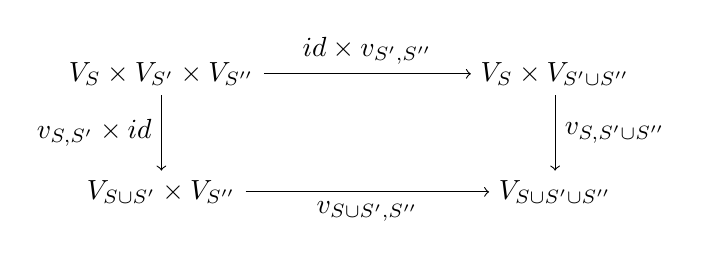
\begin{tikzpicture}
		\node (LT) at (0, 1.5) {$V_S \times V_{S'} \times V_{S''}$};
		\node (LB) at (0, 0) {$V_{S \cup S'} \times V_{S''}$};
		\node (RT) at (5, 1.5) {$V_S \times V_{S' \cup S''}$};
		\node (RB) at (5, 0) {$V_{S \cup S' \cup S''}$};
		\draw [->] (LT) -- node [left] {$v_{S,S'} \times id$} (LB);
		\draw [->] (LT) -- node [above] {$id \times v_{S', S''}$} (RT);
		\draw [->] (RT) -- node [right] {$v_{S, S' \cup S''}$} (RB);
		\draw [->] (LB) -- node [below] {$v_{S \cup S', S''}$} (RB);
		%\node at (0.5, 1) {$\ulcorner$};
		%\node at (1.5, 0.5) {$\lrcorner$};
	\end{tikzpicture}
	\end{center}
	\end{enumerate} 
	\item The morphisms from $\{ V_S, v_{S, S'} \} \to \{ W_S, w_{S, S'} \}$ consist of collections of linear maps $\{ \phi_S: V_S \to W_S \}$, such that $\phi_{\emptyset} = id$ and for each pair of disjoint subsets $S, S' \subseteq B$ the following square commutes:
	\begin{center}
	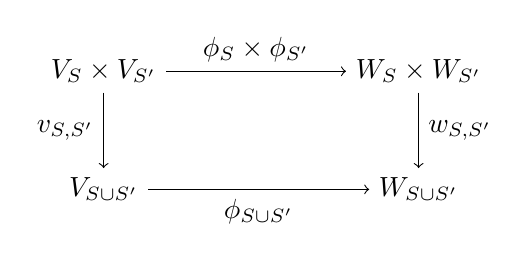
\begin{tikzpicture}
		\node (LT) at (0, 1.5) {$V_S \times V_{S'}$};
		\node (LB) at (0, 0) {$V_{S \cup S'}$};
		\node (RT) at (4, 1.5) {$W_S \times W_{S'}$};
		\node (RB) at (4, 0) {$ W_{S \cup S'}$};
		\draw [->] (LT) -- node [left] {$v_{S,S'}$} (LB);
		\draw [->] (LT) -- node [above] {$\phi_S \times \phi_{S'}$} (RT);
		\draw [->] (RT) -- node [right] {$w_{S,S'}$} (RB);
		\draw [->] (LB) -- node [below] {$\phi_{S \cup S'}$} (RB);
		%\node at (0.5, 1) {$\ulcorner$};
		%\node at (1.5, 0.5) {$\lrcorner$};
	\end{tikzpicture}.
	\end{center}
\end{itemize}
Thus an object of $\Vect(A)$ consist partly of an $A$-tuple of vector spaces, namely $ (V_{\{a\}})_{a \in A}$. Each vector space $V_S$ should then be thought of as a {\em choice} of simultaneous tensor product of all the $V_{\{a\}}$ where $a \in S$. The data and conditions of an object of $\Vect(A)$ make this philosophical viewpoint precise, and similarly for the morphisms of $\Vect(A)$. 

The assignment $A \mapsto \Vect(A)$ gives a functor $\Vect: \Gamma^{op} \to \Cat$, for if $f: A \to P(B)$, then we obtain a functor $f^*: \Vect(B) \to \Vect(A)$ as follows. If $T \subseteq A$, let $f(T) = \cup_{a \in T} f(a) \subseteq B$. Then an object $\{ V_S, v_{S,S'} \}_{S, S' \subseteq B}$ of $\Vect(B)$ is sent via $f^*$ to the object $\{ W_T, w_{T, T'} \}_{T, T' \subseteq A} \in \Vect(A)$, where 
\begin{equation*}
	W_T = V_{f(T)} \quad \textrm{and} \quad  w_{T, T'} = v_{f(T), f(T')}.
\end{equation*}
This is easily seen to be strictly compatible with composition in $\Gamma^\text{op}$. Moreover, since the tensor product is defined by a universal property, the forgetful functor $\Vect(A) \to \Vect^{\times |A|}$ is an equivalence of categories, as desired.  

\section{Composition via the category $\Delta$}


\NS{As discussed in email, this subsection should have an expository paragraph near the beginning incorporating some of the motivational material currently in the next section}

In the last section we described how symmetric monoidal structures may be encoded through the use of the category $\Gamma$. In this section we will describe a similar process in which the composition in a category may be described through the use the combinatorial simplex category $\Delta$. Iterating this idea leads to the notion of {\em $n$-fold Segal category}, and incorporating our insights about $\Gamma$ yields a notion of symmetric monoidal $(\infty,3)$-category.  

\begin{definition}
	The simplex category $\Delta$ is a skeleton of the category of finite non-empty totally ordered sets and order preserving maps. The objects of $\Delta$ are the ordered sets $[n] = \{ 0 < 1 < 2 < \cdots < n\}$. 
\end{definition}

The simplex category plays a dual role which sometimes results in confusing terminology. On the one had it has a geometric interpretation as the category of combinatorial simplices. This gives rise to terminology such as a {\em $k$-simplex} of $[n]$, which is a strictly order preserving map $[k] \to [n]$. There are $ {n+1}\choose {k+1}$ such maps. The $0$-simplices will be called {\em vertices} and $1$-simplices will be called {\em edges}. 

But there are other aspects of $\Delta$ which come from its description as a category of certain totally ordered sets. The vertices of $[n]$ have a natural ordering induced from the ordering of $[n]$. Let $[m + n]$ denote the ordered concatenation of $[m]$ with $[n]$. We thus obtain the following commuting square,
\begin{equation} \label{Eqn:Segal-Co-Map}
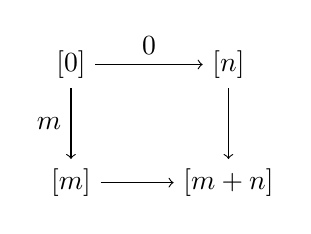
\begin{tikzpicture}[baseline = 0.75cm]
	\node (LT) at (0, 1.5) {$[0]$};
	\node (LB) at (0, 0) {$[m]$};
	\node (RT) at (2, 1.5) {$[n]$};
	\node (RB) at (2, 0) {$[m+n]$};
	\draw [->] (LT) -- node [left] {$m$} (LB);
	\draw [->] (LT) -- node [above] {$0$} (RT);
	\draw [->] (RT) -- node [right] {$$} (RB);
	\draw [->] (LB) -- node [below] {$$} (RB);
	%\node at (0.5, 1) {$\ulcorner$};
	%\node at (1.5, 0.5) {$\lrcorner$};
\end{tikzpicture}
\end{equation}
where $0: [0] \to [n]$ and $m: [0] \to [m]$ denote the first and last vertices, respectively. This square will play an important role in what follows. 

Just as a monoid may be described as a certain presheaf on $\Gamma$, a category may be described as a certain presheaf on $\Delta$, called the {\em nerve} of the category. This well-known construction proceeds as follows: each of ordered sets $[n] \in \Delta$ may be viewed as a category (the objects are the elements of $[n]$, with a unique morphism from $i$ to $j$ is $i \leq j$). Thus if $X$ is a category, we obtain a presheaf $NX$ of sets on $\Delta$ by the assignment $[n] \mapsto NC_n = Fun([n], X)$, the set of functors from $[n]$ to $X$.    
The $n^\textrm{th}$ set of $NX_{\bullet}$ is given by the formula
\begin{equation*}
	NX_n := \sqcup_{x_0, x_1, \dots, x_n \in X_0} \Hom_X(x_0, x_1) \times \Hom_X(x_1, x_2) \times \cdots \times \Hom_X(x_{n-1}, x_n).
\end{equation*}
In other words $NC_n$ consists of all length $n$ strings of composable morphisms of $X$.

The nerve construction $N$ is a fully-faithful functor from categories and functors to the category of presheaves. Moreover the essential image of the nerve construction consists of those presheaves $X$ on $\Delta$  such that the squares induced by those in equation (\ref{Eqn:Segal-Co-Map}),
\begin{center}
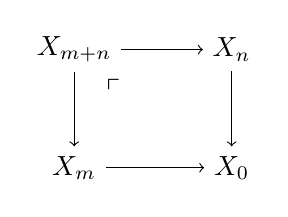
\begin{tikzpicture}
	\node (LT) at (0, 1.5) {$X_{m+n}$};
	\node (LB) at (0, 0) {$X_m$};
	\node (RT) at (2, 1.5) {$X_n$};
	\node (RB) at (2, 0) {$X_0$};
	\draw [->] (LT) -- node [left] {$$} (LB);
	\draw [->] (LT) -- node [above] {$$} (RT);
	\draw [->] (RT) -- node [right] {$$} (RB);
	\draw [->] (LB) -- node [below] {$$} (RB);
	\node at (0.5, 1) {$\ulcorner$};
	%\node at (1.5, 0.5) {$\lrcorner$};
\end{tikzpicture}
\end{center}
are a pullback diagrams. 

This can be extended to categories internal to a category $C$. The category of {\em simplicial objects of $C$} is the functor category $Fun(\Delta^\textrm{op}, C) = sC$. We write $X_\bullet$ for such a functor, and let $X_n$ denote the value assigned $[n] \in \Delta$. A {\em category internal to $C$}\footnote{This is easily checked to be equivalent to the standard definition.} is a simplicial object $X$, such that the diagrams induced by those in equation (\ref{Eqn:Segal-Co-Map}),
\begin{center}
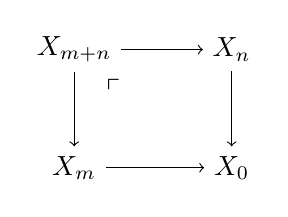
\begin{tikzpicture}
	\node (LT) at (0, 1.5) {$X_{m+n}$};
	\node (LB) at (0, 0) {$X_m$};
	\node (RT) at (2, 1.5) {$X_n$};
	\node (RB) at (2, 0) {$X_0$};
	\draw [->] (LT) -- node [left] {$$} (LB);
	\draw [->] (LT) -- node [above] {$$} (RT);
	\draw [->] (RT) -- node [right] {$$} (RB);
	\draw [->] (LB) -- node [below] {$$} (RB);
	\node at (0.5, 1) {$\ulcorner$};
	%\node at (1.5, 0.5) {$\lrcorner$};
\end{tikzpicture}
\end{center}
are a pullback diagrams. For a general simplicial object $X$, these commuting squares will be called {\em Segal squares} and if they are pullback squares we will say that $X$ satisfies the {\em Segal condition}. Hence a category internal to $C$ is a simplicial object satisfying the Segal condition. 

This may be contrasted with the notion of a category enriched to $C$, which consists of a {\em set} of objects together with hom objects $\Hom(x,y) \in C$ (as opposed to an object $X_0 \in C$ of objects). Under certain conditions these notions may be related. Recall that a category is {\em extensive} (or {\em infinitary extensive}) if it admits small coproducts and coproducts are disjoint and stable under pullback. If $C$ is an extensive category with a terminal object, then a category enriched in $C$ is merely an internal category $X$ in which the object $X_0$ is {\em discrete}, i.e. a coproduct of terminal objects. Examples of extensive categories with terminal objects include the categories of sets, any category of presheaves (or more generally any Grothendieck topos), the category of topological spaces, and the category of small categories. 

\begin{example}
	An ordinary (small) category is a category enriched in sets.
\end{example}

\begin{example}
	A {\em strict 2-category} is a category enriched in categories.
\end{example}

Thus a strict 2-category may equivalently be regarded as a simplicial object with values in $\Cat$, such that $X_0$ is a set (thought of as a discrete category), and such the the Segal squares are pullback squares. Since $X_0$ is a set, these pullbacks may be simultaneously regarded as pullbacks in the 1-category of categories and functors or as weak (or homotopy) pullbacks in the 2-category of categories, functors, and natural transformations. If $X_0$ is allowed to be a general category, these two notions of pullback may differ. 

\section{Symmetric monoidal $(\infty,n)$-categories} \label{sec-symmoninftyNcat}


We would now like to use this to insight to describe higher categories. Philosophically an $n$-category is a category enriched in $(n-1)$-categories, and so we should be able to describe it as a presheaf on $\Delta$ with values in the category of $(n-1)$-categories. Moreover this should mimic the nerve. The element $[n] \in \Delta$ should be mapped to the $(n-1)$-category of all length $n$ composable strings of $1$-morphisms. 

However, unless our $n$-category is strict this naive attempt will fail to produce a functor out of $\Delta$. The reasons are completely analogous to the previous situation of symmetric monoidal structures. However, the insight gained from the previous section also suggests a possible solution. Rather then require $X_{m+n}$ to be {\em isomorphic} to the pullback $X_m \times_{X_0} X_n$, we require that it merely be {\em equivalent} to the pullback. 
\CSP{Get references/check references for this.}
Following this reasoning gives rise to the notion of weak $n$-category constructed by Simpson and Tamsamani. In what follows we will describe $(\infty,n)$-versions of this construction, where sets are replaced by spaces.  

\begin{definition}
	Let $\sSet$ denote the category of simplicial sets. An {\em $n$-fold simplicial space} is a functor $X: (\Delta^\textrm{op})^{\times n} \to \sSet$. A {\em $\Gamma$-$n$-fold simplicial space} is a functor $X: \Gamma^\textrm{op} \times (\Delta^\textrm{op})^{\times n} \to \sSet$.
\end{definition}

The categories of $n$-fold simplicial spaces and $\Gamma$-$n$-fold simplicial spaces admit combinatorial model structures which give robust theories of $(\infty, n)$-categories and symmetric monoidal $(\infty, n)$-categories, respectively. 
\CSP{Find reference.}
The Hopkins-Lurie proof of the cobordism hypothesis has been proven using this machinery, and so it is natural to  frame our results in this language as well. The fibrant objects of these model categories are the so-called $n$-fold complete Segal spaces and symmetric monoidal $n$-fold complete Segal spaces, respectively (these later are sometimes called special $\Gamma$-$n$-fold complete Segal spaces).
These fibrant objects enjoy many desirable properties. For example, the weak equivalences between fibrant objects are precisely the levelwise weak equivalences. Also many related constructions, like the homotopy category of an $(\infty, n)$-category, have simple direct descriptions for these fibrant objects. 

On the other hand, many examples occurring { in nature} do not arise as $n$-fold complete Segal spaces or as symmetric monoidal $n$-fold complete Segal spaces. For example in \cite{MR2555928}, the $(\infty, n)$-category of cobordisms is constructed as a $n$-fold Segal space which is {\em not} complete. There are a number of classes of $n$-fold simplicial spaces which are intermediary between general $n$-fold simplicial spaces and the fibrant $n$-fold complete Segal spaces. For many purposes these intermediary objects are just as good as their fibrant replacement. One such intermediate notion is that of $n$-fold Segal category, and it is this intermediate notion to which we now turn. 
%\begin{definition}
%	An $n$-fold simplicial space $X$ is {\em essentially constant} if, when regarded as a functor $X: (\Delta^\textrm{op})^{\times n} \to h\textrm{-}(sSet)$, it is equivalent to a constant functor, where $h\textrm{-}(sSet)$ denotes the homotopy category of simplicial sets.  
%\end{definition}
%
We may regard any $n$-fold simplicial space as a simplicial object in $(n-1)$-fold simplicial spaces. A $0$-fold simplicial space is understood to be a simplicial set.

\begin{definition}
	A $0$-fold simplicial space (i.e. a simplicial set) is a {\em $0$-fold Segal category} if it is a Kan complex. An $n$-fold simplicial space $X$, regarded as a simplicial object $X_\bullet$ in $(n-1)$-fold simplicial spaces is an {\em $n$-fold Segal category} if the following conditions are satisfied
		\begin{enumerate}
			\item The $(n-1)$-fold simplicial space $X_0$ is constant and discrete.
			\item Each of the $(n-1)$-fold simplicial spaces $X_k$ is an $(n-1)$-fold Segal category.
			\item For every $m, k$, the Segal square,
			\begin{center}
			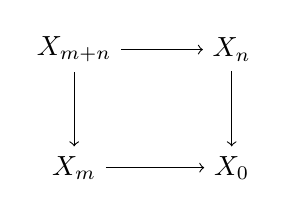
\begin{tikzpicture}
				\node (LT) at (0, 1.5) {$X_{m+n}$};
				\node (LB) at (0, 0) {$X_m$};
				\node (RT) at (2, 1.5) {$X_n$};
				\node (RB) at (2, 0) {$X_0$};
				\draw [->] (LT) -- node [left] {$$} (LB);
				\draw [->] (LT) -- node [above] {$$} (RT);
				\draw [->] (RT) -- node [right] {$$} (RB);
				\draw [->] (LB) -- node [below] {$$} (RB);
				%\node at (0.5, 1) {$\ulcorner$};
				%\node at (1.5, 0.5) {$\lrcorner$};
			\end{tikzpicture}
			\end{center}
			is a homotopy pull-back square of $(n-1)$-fold simplical spaces, computed with the $(\infty, n-1)$-model structure.
		\end{enumerate}
	\end{definition}
This final condition requires some explanation. The Segal square must realize $X_{m+n}$ as the homotopy fiber product $X_m \times_{X_0}^h X_n$, and this homotopy fiber product must be computed in the $(\infty, n-1)$-category model structure on $(n-1)$-fold simplicial sets. Moreover $X_{m+n}$ may not be levelwise equivalent to this homotopy fiber product, but merely weakly equivalent in this model structure. Fortunately, we require that $X_0$ is a discrete $(n-1)$-fold simplicial space. In this case the homotopy fiber product simplifies and is merely the ordinary fiber product. Thus condition (3) is equivalent to:

\begin{enumerate}
	\item [(3')] For every $m$ and $k$ the Segal map $X_{m+n} \to X_m \times_{X_0} X_n$ is an equivalence of $(n-1)$-fold Segal categories. 
\end{enumerate}

Moreover equivalences between $n$-fold Segal categories admit a fairly tractable inductive recognition principle. To describe this me must introduce a few auxiliary concepts. Let $X$ be an $n$-fold Segal category. Recall that $X_0$ is a constant discrete simplicial space, and so may be regarded as a set. We call the elements of $X_0$ objects of $X$. 
Inductively we will define three functorial constructions:
\begin{itemize}
	\item For every pair of objects $a,b \in X_0$, an $(n-1)$-fold Segal category $\Hom_X(a,b)$.
	\item A category $\mathit{h}X$, called the {\em homotopy category} of $X$.
	\item A set $\pi_0 X$, which is the set of isomorphism classes of objects of $\mathit{h}X$. 
\end{itemize}
Once we have these constructions, equivalences of $n$-fold Segal categories are easily recognized: they are precisely those maps $f:X \to Y$ of $n$-fold simplicial spaces which induce bijections $\pi_0 f: \pi_0 X \to \pi_0 Y$, 
% equivalences of homotopy categories $\mathit{h}f:\mathit{h}X \to \mathit{h}Y$ 
and which induce equivalences of $(n-1)$-fold Segal categories $\Hom_X(a,b) \to \Hom_Y(fa, fb)$ for every pair of objects $a,b \in X_0$. Such maps also induce equivalences $\mathit{h}f:\mathit{h}X \to \mathit{h}Y$.

Given a pair objects $a,b \in X_0$ in an $n$-fold Segal category $X$, the $(n-1)$-fold Segal category $\Hom_X(a,b)$ is defined to be the fiber over $(a,b) \in X_0 \times X_0$ of the map $(d_0, d_1): X_1 \to X_0 \times X_0$.  
\begin{center}
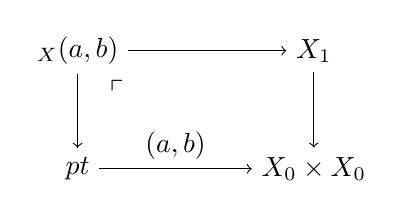
\begin{tikzpicture}
	\node (LT) at (0, 1.5) {$\Hom_X(a,b)$};
	\node (LB) at (0, 0) {$pt$};
	\node (RT) at (3, 1.5) {$X_1$};
	\node (RB) at (3, 0) {$X_0\times X_0$};
	\draw [->] (LT) -- node [left] {$$} (LB);
	\draw [->] (LT) -- node [above] {$$} (RT);
	\draw [->] (RT) -- node [right] {$$} (RB);
	\draw [->] (LB) -- node [above] {$(a,b)$} (RB);
	\node at (0.5, 1) {$\ulcorner$};
	%\node at (1.5, 0.5) {$\lrcorner$};
\end{tikzpicture}
\end{center}
The homotopy category $\mathit{h}X$ has the same object set $X_0$, and the morphisms set between two objects is given as the set $\Hom_{\mathit{h}X}(a,b) := \pi_0 \Hom_X(a,b)$. For every triple of objects $a,b,c \in X_0$ we have a similar $(n-1)$-fold Segal category $\Hom_X(a,b,c)$ which is defined as the fiber in $X_2$ over the point $(a,b,c)$ in $X_0 \times X_0 \times X_0$. Since $X$ is an $n$-fold Segal category we have induced maps of $(n-1)$-fold Segal categories,
\begin{equation*}
	\Hom_X(a,b) \times \Hom_X(b,c) \stackrel{\simeq}{\longleftarrow} \Hom_X(a,b,c) \stackrel{}{\longrightarrow} \Hom_X(a,c).
\end{equation*}
Composition in $\mathit{h}X$ is given by the induced map of sets,
\begin{equation*}
	 \Hom_{\mathit{h}X}(a,b) \times \Hom_{\mathit{h}X}(b,c) \cong \pi_0 \Hom_X(a,b,c)\to \pi_0 \Hom_X(a,c) = \Hom_{\mathit{h}X}(a,c).
\end{equation*}

\begin{example}
	If we regard a set as a constant simplicial space, then the nerve of a category $NC$ is a 1-fold Segal category. $NC_0 = \textrm{ob}\ C$ and the space $\Hom_{NC}(a,b)$ are the sets $\Hom_C(a,b)$. Moreover $hNC \cong C$ is isomorphic to the category $C$. 
\end{example}

\begin{example}
	A strict 2-category $C$ may be regarded as a simplical object $C_\bullet$ in $\Cat$ whose $n^\textrm{th}$ category is given by the usual formula
	\begin{equation*}
		C_n := \sqcup_{x_0, x_1, \dots, x_n \in C_0} \Hom_C(x_0, x_1) \times \Hom_C(x_1, x_2) \times \cdots \times \Hom_C(x_{n-1}, x_n).
	\end{equation*}
	We obtain a 2-fold simplicial set by applying the nerve construction to each of these categories, which, by viewing a set as a discrete simplicial space, we regard as a 2-fold simplicial space $NC_{\bullet \bullet}$. Since $C_\bullet$ satisfies the Segal condition, one deduces that $NC_{\bullet \bullet}$ is a 2-fold Segal category. 
	\footnote{Alternatively, one may start with the simplicial category $C_\bullet$, as before and apply the {\em complete Segal space nerve} to each of the categories $C_n$. The $k^\text{th}$ space of this simplicial space $N^{CSS}_\bullet C_n$ is obtained by first constructing the functor category $Fun([k], C_n)$, then throwing away the non-invertible natural transformations, and finally applying the classifying space functor to the resulting groupoid. This alternative has the advantage that it produces a {\em complete} Segal space $N^{CSS} C_n$. However for our purposes these are equivalent constructions as the canonical map $N C_n \to N^{CSS} C_n$ is a weak equivalence in the complete Segal space model structure. 
	%[Cite the Joyal Teinery paper for the Quillen equivalence between Segal spaces and Quasi-categories]
	} We call the association $C \mapsto NC_{\bullet \bullet}$ the {\em 2-categorical nerve}. 
	\CSP{We should get a reference for this.}
\end{example}

\begin{lemma} \label{lma:2catnervereflectsequiv}
	A strict functor of strict 2-categories $F: C \to D$ is a weak equivalence if and only if the induced map of 2-fold Segal categories $NC_{\bullet \bullet} \to ND_{\bullet \bullet}$ is an equivalence. 
\end{lemma}

\begin{proof}
	The functor $F$ is a weak equivalence if and only if 
	\begin{enumerate}
		\item it is essentially surjective on object, and
		\item for every pair of objects $a,b \in C$,  it induces an equivalence of categories $C(a,b) \to D(Fa, Fb)$.
	\end{enumerate}
On the other hand, a map of 2-fold Segal spaces $X \to Y$ is an equivalence if and only if
\begin{enumerate}
	\item it induces a bijection $\pi_0X \to \pi_0Y$, and
	\item for every pair of objects $a,b \in X_0$, it induces equivalences of 1-fold Segal spaces $\Hom_X(a,b) \to \Hom_Y(Fa, Fb)$.
\end{enumerate}
When $X = NC_{\bullet \bullet}$  is a 2-categorical nerve, $\Hom_X(a,b) \cong NC(a,b)_{\bullet}$, so the second conditions are equivalent. Moreover, $\pi_0 NC_{\bullet \bullet}$ is easily seen to be the collection of equivalence classes of objects of $C$. Thus a functor inducing an equivalence of 2-categorical nerves induces a bijection on equivalence classes of objects. In particular if $F$ induces an equivalence of 2-categorical nerves, it is essentially surjective, and hence a weak equivalence of categories. It remains to see that a weak equivalence of categories necessarily induces a bijection on sets of equivalence classes of object. This follows as a well-known exercise.
\end{proof}

%If the $n$-fold Segal spaces $X_k$ are fibrant, that is complete, then these problems disappear. Weak equivalences between fibrant objects are computed levelwise, as are homotopy fiber products. 

%Thus in general we are left with the embarrassing responsibility of computing the correct homotopy fiber product $X_m \times_{X_0}^h X_n$, and showing that the canonical map from $X_{m+n}$ is a weak equivalence of $(\infty, n-1)$-categories. Fortunately there is another subclass of $n$-fold Segal spaces for which these two operations are relatively easy to perform: The {\em $n$-fold Segal categories}.

\begin{definition}
%   A $0$-fold Segal category is a Kan complex. An {\em $n$-fold Segal category} is an $n$-fold Segal space which satisfies
%   \begin{enumerate}
%   	\item $X_0$ is discrete, and
%   	\item for each $n$, $X_n$ is an $(n-1)$-fold Segal category. 
%   \end{enumerate}
	A {\em symmetric monoidal $n$-fold Segal category} (a.k.a. {\em special $\Gamma$-$n$-fold Segal category}) is a $\Gamma$-$n$-fold simplicial space $X$, which we view as a functor from $\Gamma^\textrm{op}$ to $n$-fold simplicial spaces, such that the following conditions are satisfied. 
	\begin{enumerate}
		\item $X_A$ is an $n$-fold Segal category for each $A \in \Gamma$. 
		\item For each set $A \in \Gamma$ (possibly empty) the canonical map,
		\begin{equation*}
			\prod_{a \in A} i_a^*: X_A \to \prod_{a \in A} X_{(1)}
		\end{equation*}
		is an equivalence of $n$-fold Segal categories. %\CSP{Should we also add the $X_{(0)} = pt$? We get $X_{(0)} \simeq pt$ for free.}
	%	\item (optional) The previous axiom implies that $X_\emptyset \simeq pt$. We assert that $X_\emptyset = pt$. 
	\end{enumerate}
\end{definition}


\section{Dualizability in Symmetric Monoidal 3-Categories}

In the next section we will construct several examples describing versions of the symmetric monoidal 3-fold Segal category of tensor categories. 

%Thus the goal of this section is to describe $\TC$ as a functor $\Gamma^{\op} \times (\Delta^{\op})^{\times 3} \to \sSet$. This is done in two stages. First we construct a nerve functor from the category of strict 2-categories to 2-fold Segal categories. This reduces the construction of $\TC$ to constructing a functor (also denoted $\TC$) from $\Gamma^{\op} \times \Delta^{\op}$ to the category of strict 2-categories and strict functors. As a warm-up, we first describe a functor $\lincat$ from $\Gamma^{\op}$ to strict 2-categories which serves as a model for the symmetric monoidal 2-category of linear categories. The functor $\TC$ is a more elaborate variation on this construction. 

%We now describe how a strict 2-category gives rise to a 2-fold Segal category. This can be regarded as a 2-categorical nerve. %Later we will construct explicitly $\TC$ as a simplicial object in the category of strict 2-categories. Applying the previous 2-categorical nerve yields a 3-fold simplicial space which is shown to be a 3-fold Segal category. A variation on these constructions yields the $\Gamma$-3-fold Segal space $\TC$. 
%\begin{definition}
%	A strict 2-category is a category object $(C_1 \rightrightarrows C_0)$ in categories such that the category of objects $C_0$ is discrete (i.e. its only morphisms are identities). 
%\end{definition}
%A strict 2-category gives rise to a simplicial category 

\CSPcomm{[...] Explain the fully-dualizable filtration, and 
how the various 2-categories that one extracts from a symmetric monoidal 3-category (Segal 3-category) are invariant under completion.}







\section{Linear categories and tensor categories} \label{sec-tc-lincat}

	Let $k$ be a fixed ground field, let $\overline{\Vect}_k$ be the category of (possibly infinite dimensional) $k$-vector spaces, and $\Vect_k$ be the category of finite dimensional $k$-vector spaces.   A {\em linear category} is an abelian category with a compatible enrichment over $\overline{\Vect}_k$, the category of (possibly infinite dimensional) $k$-vector spaces. 
A {\em linear functor} is a right exact additive functor, which is also a functor of $\overline{\Vect}_k$-enriched categories. 
	
More generally if $\{\cA_\alpha\}$ denotes a collection of linear categories then a {\em multilinear functor} from $\{\cA_\alpha\}$ into a linear category $\cB$ consists of a functor
\begin{equation*}
	F: \prod \cA_\alpha \to \cB
\end{equation*}
such that $F$ is linear in each variable separately. A linear category will be said to {\em have enough projectives} if every simple object has a projective cover. 

\begin{warning}
	Unless otherwise stated {\em all linear functors considered in this paper are {\bf right exact} functors}.  We are aware that this deviates from convention, and offer the following justification. Many of the construction that will be described in this paper, such as the Deligne tensor product of linear categories and the composition of bimodule categories, are only functorial with respect to right exact functors. To avoid littering this paper with the adjective `right exact' it is simpler to define right exactness into the category from the start.  
\end{warning}

\begin{definition}
	A {\em tensor category} is a linear monoidal category $(\cC, \otimes, 1, \alpha, \lambda, \rho)$ such that the functor $\otimes$ is multilinear. A {\em tensor functor} is a monoidal functor which is also linear.
\end{definition}

\begin{example}
	Both $\overline{\Vect}_k$ and $\Vect_k$ (the category of finite dimensional vector spaces) are examples of tensor categories. If $A$ is an algebra in $\Vect_k$, then the categories of finitely presented left and right modules, $\Mod{A}{}$ and $\Mod{}{A}$, are linear categories. More generally, if $\cC$ is a tensor category and $A$ is an algebra object in $\cC$ (also known as a monoid object), then the categories $\Mod{A}{}(\cC)$ and $\Mod{}{A}(\cC)$ of left and right $A$-module objects in $\cC$ are also linear categories.
\end{example}

\begin{example}
	If $\cM$ is a linear category, then the category of (right exact) linear endofunctors $\Fun(\cM, \cM)$ is a tensor category. 
\end{example}



\section{Bimodule categories} \label{sec-tc-bimodcat}

\begin{definition}
	Let $\cC$ and $\cD$ be tensor categories. A {\em $\cC$-$\cD$-bimodule category} is a bicategory with two objects $x$ and $y$ such that
	\begin{itemize}
		\item all hom categories are linear categories, 
		\item horizontal composition is multilinear, and
		\item there are identifications of monoidal categories $\Hom(x,x) \simeq \cD$, $\Hom(y,y) \simeq \cC$, and $\Hom(y,x) \simeq \emptyset$.
	\end{itemize}
	We will often abuse notation and refer to the value $\cM = \Hom(x,y)$ as the bimodule category. If $\cD \simeq \Vect_k$, then $\cM$ is a {\em left module category}. If $\cC \simeq \Vect_k$, then $\cM$ is a {\em right module category}.
\end{definition}
	
Unwrapping this definition we see that a left $\cC$-module category is a linear category $\cM$ together with a multilinear functor $\otimes^{\cM}: \cC \times \cM \to \cM$ and natural isomorphisms
%	\CSP{This looks a little gross. I should change it.}
	\begin{align*}
		\alpha: & \;    \otimes^{\cM} \circ (\otimes \times id_{\cM}) \cong  \otimes^{\cM} \circ (id_{\cC} \times \otimes^{\cM}) \\
		\lambda: & \; 1 \otimes^{\cM}(-) \cong id_{\cM},
	\end{align*}
%	\begin{align*}
%		\alpha: & \;    [(-) \otimes (-)] \otimes^{\cM} (-)  \cong  (- ) \otimes^{\cM} [ (-) \otimes^{\cM} (-)] \\
%		\lambda: & \; 1 \otimes^{\cM}(-) \cong id_{\cM},
%	\end{align*}	
	satisfying the evident pentagon and triangle identities. 

\begin{definition}		
A {\em $\cC$-$\cD$ bimodule functor} $F:\cM \to \cN$ is a (strong) functor of bicategories such that 
%	\begin{itemize}
		 $F$ is the identity on objects,
		  the restriction of $F$ to each hom category is linear,
		 and $F$ is the identity on $\Hom(x,x)$ and $\Hom(y,y)$.
%	\end{itemize}
A {\em lax} (resp. {\em oplax}) bimodule functor is a lax (resp. oplax) functor of bicategories satisfying the above conditions. All bimodule functors will be assumed strong unless otherwise stated. 
	A {\em bimodule transformation} is a transformation of functors of bicategories, which restricts to the identity on $\Hom(x,x)$ and $\Hom(y,y)$, and such that the component 1-cells are trivial.  
\end{definition}
	
%
Bimodule categories, functors, and transformations form a strict 2-category.
%If $\cM$ and $\cN$ are both $\cC$-$\cD$ bimodule categories, then a bimodule functor which restricts to the identity functor on $\cC$ and $\cD$ will be called a {\em $\cC$-$\cD$-bimodule functor}.

\begin{example}
	Every linear category is a $\Vect_k$-$\Vect_k$-bimodule category in an essentially unique way. 
\end{example}

\begin{example}
	For any algebra object $A$ in a tensor category $\cC$ the categories $\Mod{}{A}(\cC)$ and $\Mod{A}{}(\cC)$ are respectively left and right $\cC$-module categories. 
\end{example}

\begin{example}
	Let $\cM$ and $\cN$ be left $\cC$-module categories. The categories $\Fun_{\cC}(\cM, \cM)$ and $\Fun_{\cC}(\cN, \cN)$ of (right exact) $\cC$-module endofunctors is a tensor category. The linear category $\Fun_{\cC}(\cM, \cN)$ is a $\Fun_{\cC}(\cN, \cN)$-$\Fun_{\cC}(\cM, \cM)$-bimodule category. 
	%\CSP{Do I have the right convention for the actions here?} \NS{I think you got it backwards.  $\Fun(\cM,\cM)$ left acts on $\cM$ and so its action by precomposition should be a right action} 
\end{example}

\begin{remark}
 	Every left $\cC$-module category is naturally a right $\cC^{mp}$-module category. 
\end{remark}

We will also need a slightly more general notion of bimodule morphism to make sense of multilinear bimodule maps. These in turn are used to define the external Deligne tensor product of bimodule categories and, later,  in defining the symmetric monoidal 3-category of tensor categories. 

\begin{definition}
	A {\em twisted bimodule functor} from a $\cC$-$\cD$-bimodule category $\cM$  to $\cC'$-$\cD'$-bimodule category $\cM'$ is a functor of bicatgories from $\cM$ to $\cM'$ which restricts to the identity on objects and is linear on hom categories. A {\em twisted bimodule transformation} between twisted bimodule functors is a transformation of functors of bicategories such that the component 1-cells are trivial.
\end{definition}

Thus a twisted bimodule functor from a $\cC$-$\cD$-bimodule category $\cM$ to a $\cC'$-$\cD'$-bimodule category $\cM'$ consists in part of tensor functors $f:\cC \to \cC'$ and $g:\cD \to \cD'$, and a map of linear categories $\cM \to \cM'$, compatible with the induced module structures. We will say the the twisted bimodule functor {\em extends the tensor functors $f$ and $g$}. 

If we are given a $\cC'$-$\cD'$-bimodule category $\cM'$ and tensor functors $f:\cC \to \cC'$ and $g:\cD \to \cD'$, then we may also form the {\em twisted bimodule category} ${}_f{\cM'}_g$.  The underlying linear category of ${}_f{\cM'}_g$ is $\cM'$, but the actions are by $\cC$ and $\cD$ via the tensor functors $f$ and $g$. A twisted bimodule functor $\cM \to \cM'$ extending $f$ and $g$ is the same as a $\cC$-$\cD$-bimodule functor $\cM \to {}_f{\cM'}_g$.  Later on we will sometimes use the notation ${}_{\langle f \rangle} \cM'_{\langle g \rangle}$ instead of ${}_f{\cM'}_g$, in cases where the functors $f$ and $g$ are themselves unwieldy composites.

With twisted bimodule functors as morphisms, there exists a terminal bimodule category $\cT$. As a bicategory, each of its non-empty hom categories is the terminal linear category. The product of bimodule categories $\cM \times_{\cT} \cM'$ is defined as the fiber product of bicategories over $\cT$. We will abuse notation and write this as $\cM \times \cM'$. This is again a bicategory with precisely two objects $x$ and $y$. Moreover
\begin{equation*}
	\Hom_{\cM \times \cM'}(a,b) = \Hom_\cM(a,b) \times \Hom_{\cM'}(a,b)
\end{equation*}
for all pairs $a,b \in \{ x,y \}$.

If $\{ \cM_\alpha \}$ is a collection of bimodule categories then a {\em twisted multilinear bimodule functor} from $\{ \cM_\alpha \}$ into a bimodule category $\cN$ is a functor of bicategories
\begin{equation*}
	\prod_{\alpha} \cM_\alpha \to \cN
\end{equation*}
which is the identity on objects, and which is a twisted bimodule functor in each variable. 

\section{The Deligne tensor product and finite linear categories} \label{sec-tc-deligne}

The goal of this section is to construct the Deligne tensor product, which takes module categories $\cM_\cC$ and ${}_\cC \cN$ and returns a linear category $\cM \boxtimes_\cC \cN$.  This tensor product only makes sense for categories satisfying certain smallness properties, so we first introduce the notion of finite tensor categories and discuss their properties.

\begin{definition} % This is from EGNO Definition 1.18.2.
	A linear category $\cC$ is {\em finite} if 
	\begin{enumerate}
		\item $\cC$ has finite dimensional spaces of morphisms;
		\item every object of $\cC$ has finite length;
		\item $\cC$ has enough projectives, i.e. every simple object of $\cC$ has a projective cover; and
		\item there are finitely many isomorphism classes of simple objects.  
	\end{enumerate}
\end{definition}

\begin{remark}
A linear category is finite if and only if it is equivalent to the category $\Mod{A}{}$ of finite dimensional modules over a finite dimensional $k$-algebra $A$.
\end{remark}

The key property of finite tensor categories is that they satisfy the following analog of the adjoint functor theorem.  Although this result is well known, we were unable to find a proof in the literature, so we sketch the proof here.

\begin{proposition} \label{prop:AFT}
	Let $\cC$ and $\cD$ be finite linear categories and let $\cG: \cC \rightarrow \cD$  be an additive $\Vect$-enriched functor (not necessarily right exact). Then the following conditions are equivalent:
	\begin{enumerate}
		\item $\cG$ is left exact;  
		\item $\cG$ is left exact and satisfies the following {\em Solution Set Condition:} \\  For each $d \in \cD$ there is a finite set $I$ and a collection of arrows $f_i:d \to \cG(c_i)$ such that every arrow $h:d \to \cG(c)$ can be written as a composite $h = \cG(t) \circ f_i$ for some index $i \in I$ and some $t: c_i \to c$; 
		\item $\cG$ admits an (additive, ${\Vect}$-enriched) left adjoint.
	\end{enumerate}
\end{proposition}
\begin{proof} This is a variation of the proof given in \cite[V.6.Thm 2]{MR0354798}.
Suppose that $\cG$ admits a left adjoint, $\cF$. Then $\cG$ is itself a right adjoint and hence commutes with all limits. In particular $\cG$ is a left exact functor. Moreover, as $\cF$ commutes with coproducts, it is automatically additive, and as the unit and counit maps are linear maps of vector spaces, $\cF$ is also $\overline{\Vect}$-enriched. 


To construct a left adjoint for $\cG$, it suffices (and is necessary) to construct for each $d \in \cD$ a universal arrow $d \to \cG(c)$ (i.e. initial object of the comma category $(d \downarrow \cG)$),
as the left adjoint may then be constructed pointwise as $\cF(d) = c$. To this end, fix $d \in \cD$ and suppose that $\cG$ satisfies the solution set condition. Define the element $w$ of the comma category as the product of the $d \to \cG(c_i)$. Since $\cG$ is left exact, it commutes with finite limits, and hence the forgetful functor $(d \downarrow \cG) \to \cC$ creates limits. In particular the comma category has all finite limits, and this  product exists and is given explicitly by 
\begin{equation*}
	w = \bigoplus_i f_i :  d \to \cG( \oplus_i c_i) = \bigoplus_i \cG(c_i).
\end{equation*}
The morphism spaces of $(d \downarrow \cG)$ are finite dimensional vector spaces, and so we may choose a finite basis for $\Hom(w,w)$. Let $v$ be defined as the equalizer of this finite collection of maps. Again, this finite limit exists and may be created in $\cC$. By construction $v$ actually equalizes {\em all} endomorphisms of $w$, and thus by a straightforward calculation [MacLane V.6.Thm 1], we see that $v$ is initial. 

Finally, if $\cG$ is left exact, then it satisfies the solution set condition. To see this note that each object $d \in \cD$  has a finite number of distinct quotients in $\cD$, hence also a finite number quotients of the form  $\cG(c)$ for some $c \in \cC$. Thus we may choose a finite index set $I$ and objects  $c_i \in \cC$, together with maps $d \to \cG(c_i)$ exhausting the finite collection of possible quotients of $d$. Since any map $d \to \cG(c)$ must factor through one of these quotients, we have construct a solution set.   
\end{proof}

\begin{corollary}
	A linear functor between finite linear categories always admits a right adjoint (which may not be a linear functor as we have defined it; it may fail to be right exact). If the linear functor is left exact, then it also admits a left adjoint which is also a linear functor. 
\end{corollary}

\begin{proof}
	The second statement is just a rephrasing of the above proposition; the first follows by passing to the opposite linear category.  
\end{proof}


\begin{corollary}
If $\cC$ is finite, a functor $G: \cC^\textrm{op} \to \Vect$ is representable if and only if it is left exact. 
\end{corollary}

\begin{proof}
	A representable functor $\Hom(-, x):\cC^\text{op} \to \Vect$ sends all limits in $\cC^\text{op}$ (i.e. colimits in $\cC$) to limits in $\Vect$. Hence it is left exact. 
%
% 0 <-- C <--  B <--- A <-- 0 in C/C^op
% 0 -->  \Hom(c,x) ---> hom(b,x) ---> hom(a, x)
%		
Conversely, if $G: \cC^\text{op} \to \Vect$ is left exact, then by the above proposition it admits a left adjoint $F$. Thus for every every object $c \in \cC$ we have a natural isomorphism:
	\begin{equation*}
		G(c) \cong \Hom_{\Vect_k}( k, G(c)) \cong \Hom_{\cC^\op}( F(k), c) = \Hom_{\cC}(c, F(k) ).
	\end{equation*}
	In other words,  the object $F(k)$ represents the functor $G$. 
\end{proof}

Just as any finite tensor category is a category of modules over an algebra, any finite module category over a tensor category is a category of module objects over an algebra object.  This is one of the main theorems of \cite{EGNO}, and is essential to the structure theory of finite tensor categories.  The key construction underlying their proof is Ostrik's notion of the internal Hom for module categories \cite{MR1976459}.

\begin{theorem}[\cite{EGNO}] \label{thm:EGNO2.11.6} %!% [Thm 2.11.6(i)]
	Let $\cM$ be a left module category over the finite tensor category $\cC$. If $\cM$ is finite as a linear category, then there exists an algebra object $A \in \cC$ such that $\cM \simeq \Mod{}{A} (\cC)$ as left $\cC$-module categories. 
\end{theorem}

\begin{definition}
	Let $\cM$ be a right $\cC$-module category and $\cN$ a left $\cC$-module category. A {\em $\cC$-balanced functor} into a linear category $\cL$ is a multilinear functor $\cM \times \cN \to \cL$ together with a natural isomorphism $\otimes^{\cM} \times id_{\cN} \cong id_{\cM} \times \otimes^{\cN}$ satisfying the evident pentagon identity. A {\em $\cC$-balanced transformation} is a natural transformation $\eta:F \to G$ of $\cC$-balanced functors such that the following diagram commutes for all $M \in \cM$, $C \in \cC$, and $N \in \cN$:
\begin{center}
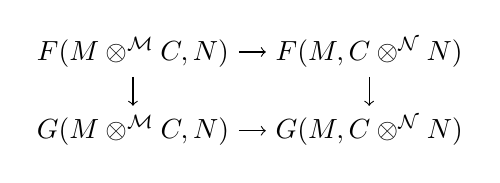
\begin{tikzpicture}
	\node (LT) at (0, 1) {$F(M \otimes^{\cM} C, N)$};
	\node (LB) at (0, 0) {$G(M \otimes^{\cM} C, N)$};
	\node (RT) at (3, 1) {$F(M, C \otimes^{\cN} N)$};
	\node (RB) at (3, 0) {$G(M, C \otimes^{\cN} N)$};
	\draw [->] (LT) -- node [left] {$$} (LB);
	\draw [->] (LT) -- node [above] {$$} (RT);
	\draw [->] (RT) -- node [right] {$$} (RB);
	\draw [->] (LB) -- node [below] {$$} (RB);
	%\node at (0.5, 1) {$\ulcorner$};
	%\node at (1.5, 0.5) {$\lrcorner$};
\end{tikzpicture}.
\end{center}
\end{definition}


\begin{definition}
	Let $\cA$ and $\cB$ be right and left $\cC$-module categories, respectively. The {\em Deligne tensor product $\cA \boxtimes_{\cC} \cB$} is the universal linear category admitting a $\cC$-balanced multilinear functor $\boxtimes_{\cC}: \cA \times \cB \to \cA \boxtimes_{\cC} \cB$. That is, there exists a $\cC$-balanced multilinear functor $\boxtimes_{\cC}: \cA \times \cB \to \cA \boxtimes_{\cC} \cB$ which induces, for all linear categories $\cD$, an equivalence between the categories of $\cC$-balanced multilinear functors $\cA \times \cB \to \cD$ and linear functors $\cA \boxtimes_{\cC} \cB \to \cD$. 
\end{definition}

If it exists, the Deligne tensor product is unique up to an equivalence, which in turn is unique up to unique natural isomorphism. Equivalently, the 2-category of linear categories representing the Deligne tensor product is either contractible or empty. 

\begin{theorem} \label{thm:DelignePrdtOverATCExists}
	Let $\cC$ be a finite tensor category and let $\cA_{\cC}$ and ${}_{\cC}\cB$ be finite right and left $\cC$-module categories, respectively. Then,
	\begin{enumerate}
		\item The Deligne tensor product $\cA \boxtimes_{\cC} \cB$ exists and is a finite linear category;
		\item If $\cA = \Mod{A}{}(\cC)$ and $\cB = \Mod{}{B}(\cC)$, then $\cA \boxtimes_{\cC} \cB \simeq \Mod{A }{B}(\cC)$;
	\end{enumerate} 
Moreover if $\cC$ is rigid, then 	
	\begin{enumerate}
		\item[(3)] The functor $\boxtimes_{\cC}$ is exact in each variable and satisfies 
		\begin{equation*}
			\Hom_{\cA}(x,x') \otimes \Hom_{\cB}(y, y') \cong \Hom_{\cA \boxtimes_{\cC} \cB} (x \boxtimes_{\cC} y, x' \boxtimes_{\cC} y'),
		\end{equation*}
		\item[(4)] If $F: \cA \times \cB \to \cD$ is a $\cC$-balanced multilinear functor which is exact in each variable, then it defines an exact functor $\overline{F}: \cA \boxtimes_{\cC} \cB \to \cD$. 
	\end{enumerate} 
\end{theorem}

\begin{proof}
	When $\cC = \Vect_k$, this is classical \cite[Prop 5.13]{MR1106898} (see also \cite[Prop 1.46.2]{EGNO}).
	By Theorem \ref{thm:EGNO2.11.6} to show (1) and (2) it is enough to assume that $\cA = \Mod{A}{}(\cC)$ and $\cB = \Mod{}{B}(\cC)$ and show that $\Mod{A }{B}(\cC)$ has the desired universal property. Tensoring a left $A$-module and a right $B$-module gives a canonical $\cC$-balanced multilinear functor 
		\begin{equation*}
			T: \Mod{A}{}(\cC) \times \Mod{}{B}(\cC) \to \Mod{A}{B}(\cC),  
		\end{equation*}
and we will show that $T$ induces an equivalence between $\cC$-balanced multilinear functors $\cA \times \cB \to \cD$ and linear functors out of $\Mod{A}{B}(\cC)$.
	
	To this end, let $F:\Mod{}{A}(\cC) \times \Mod{B}{}(\cC) \to \cD$ be a $\cC$-balanced multilinear functor.  
	There is a unique right exact linear functor $\overline F: \Mod{B}{A}(\cC) \to \cA$ such that $F = \overline{F} \circ T$ which is defined as follows. On free bimodules $A \otimes X \otimes B \cong T(A \otimes X, B)$, we necessarily have $\overline{F}(A \otimes X \otimes B) \cong F(A \otimes X, B)$. Since  every $A$-$B$-bimodule $X$ is a coequalizer of free $A$-$B$-bimodules, namely the canonical coequalizer  
	\begin{equation*}
		X \leftarrow A \otimes X \otimes B \leftleftarrows A \otimes A \otimes X \otimes B \otimes B,
	\end{equation*}
	and since $\overline{F}$ is right exact the result follows.
	
	If $\cC$ is rigid, then by Lemma \ref{lma:RigidIsExact} the functor $T = \boxtimes_{\cC}$ is exact in each variable. The formula in (3) then follows as a standard exercise in using duals. Finally let $F: \cA \times \cB \to \cD$ be a $\cC$-balanced multilinear functor which is exact in each variable and let $\overline{F}: \cA \boxtimes_\cC \cB \to \cD$ be its linear extension (which is always right exact). Since $F$ is exact in each variable, $\overline{F}$ preserves left exact sequences of free $A$-$B$-bimodules (where the maps are also free). Since every $A$-$B$-bimodule has a functorial resolution by free $A$-$B$-bimodules (coming from the above mentioned coequalizer), a diagram chase shows that $\overline{F}$ is also left exact. Hence (4) is also satisfied. 
\end{proof}


%\begin{proposition}[]
%	Let $\cA$ and $\cB$ be finite linear categories. Then,
%	\begin{enumerate}
%		\item The Deligne tensor product $\cA \boxtimes \cB$ exists and is a finite linear category;
%		\item If $\cA = \Mod{A}{}$ and $\cB = \Mod{B}{}$, then $\cA \boxtimes \cB \simeq \Mod{A \otimes B}{}$;
%		\item The functor $\boxtimes$ is exact in each variable and satisfies 
%		\begin{equation*}
%			\Hom_{\cA}(x,x') \otimes \Hom_{\cB}(y, y') \cong \Hom_{\cA \boxtimes \cB} (x \boxtimes y, x' \boxtimes y'),
%		\end{equation*}
%		\item If $F: \cA \times \cB \to \cC$ is a multilinear functor which is exact in each variable, then it defines an exact functor $\overline{F}: \cA \boxtimes \cB \to \cC$. 
%	\end{enumerate} 
%\end{proposition}


\begin{remark} \label{rmk:rigidpreservedbytensor}
	We may use the case $\cC= \Vect_k$ to rewrite part the data  of a tensor category as a linear category $\cD$ equipped with an object $1 \in \cD$ and a linear functor $\otimes: \cD \boxtimes \cD \to \cD $, together with natural transformations $\alpha$, $\lambda$, and $\rho$, as before. Moreover by Corollary \ref{cor:RigidityViaFunctors} the tensor product of two rigid tensor categories is again rigid. 
\end{remark}

\begin{remark}
	If ${}_{\cD}\cA_{\cC}$ and ${}_{\cC}\cB_{\cE}$ are bimodule categories, then the actions of $\cD$ and $\cE$ induce a $\cD$-$\cE$-module category structure on $\cA \boxtimes_{\cC} \cB$. This bimodule category satisfies the analogous universal property for $\cC$-balanced twisted bilinear bimodule functors. 
\end{remark}

\begin{lemma} \label{Lma:FunctorsAsATensorPdt}
	If $\cC$ is a finite tensor category and $\cM$ and $\cN$ are finite left $\cC$-module categories then the natural functor induces an equivalence
	\begin{equation*}
		\Fun_\cC(\cM, \cC) \boxtimes_\cC \cN \simeq \Fun_\cC(\cM,\cN).
	\end{equation*}
	Here $\Fun_\cC$ denotes the category of (right exact) $\cC$-module functors. 
	Moreover, if $\cM$ and $\cN$ are bimodule categories, then the above equivalence is a bimodule equivalence. 
\end{lemma}

\begin{proof}
	The last sentence follows since in that case the natural functor is a bimodule functor. By the Theorem \ref{thm:EGNO2.11.6}, there exist algebra objects $A, B \in \cC$ and equivalences $\cM \simeq \Mod{}{A}(\cC)$ and $\cN \simeq \Mod{}{B}(\cC)$. We show that both sides of the above equation are naturally equivalent to $\Mod{A}{B}(\cC)$, the category of $A$-$B$-bimodule objects in $\cC$. The equivalence $\Fun_\cC(\cM, \cN) \simeq \Mod{A}{B}(\cC)$ (\cite[Prop 2.12.2]{EGNO}) can be seen by mirroring the classical proof. A bimodule clearly gives rise to such a functor, and given a functor $f$, we obtain an $A$-$B$-bimodule $f(A)$. By $\cC$-linearity $f(X \otimes A) \cong X \otimes f(A)  \cong (X \otimes A) \otimes_A f(A) $ is determined on free $A$-modules. Since every object of $\cM$ may be written as a (canonical) coequalizer of free $A$-modules,
	\begin{equation*}
		M \leftarrow M \otimes A \leftleftarrows M \otimes A \otimes A
	\end{equation*} 
the functor $f$ is equivalent to the one determined by the bimodule $f(A)$. Thus the natural map  $\Mod{A}{B}(\cC) \to \Fun_\cC(\cM, \cN)$ is essentially surjective. The above argument also shows it is fully-faithful, so that $\Fun_\cC(\cM, \cN) \simeq \Mod{A}{B}(\cC)$, which in particular shows $\Fun_\cC(\cM, \cC) \simeq \Mod{}{A}(\cC)$. Now the result follows from Theorem \ref{thm:DelignePrdtOverATCExists}.
%Tensoring a left $A$-module and a right $B$-module gives a canonical $\cC$-balanced bilinear functor 
%\begin{equation*}
%	T: \Mod{A}{}(\cC) \times \Mod{}{B}(\cC) \to \Mod{A}{B}(\cC). 
%\end{equation*}
%To complete the proof we must show this induces an equivalence,
%\begin{equation*}
%	\Mod{}{A}(\cC) \boxtimes_\cC \Mod{B}{}(\cC) \simeq \Mod{B}{A}(\cC).
%\end{equation*}
%When $\cC = \Vect$, this is classical. More generally we must show that the right-hand-side has the desired universal property. For this purpose let $F:\Mod{}{A}(\cC) \times \Mod{B}{}(\cC) \to \cA$ be a $\cC$-balanced bilinear functor. There is a unique right exact linear functor $\overline F: \Mod{B}{A}(\cC) \to \cA$ such that $F = \overline{F} \circ T$ which is defined as follows. On free bimodules $A \otimes X \otimes B \cong T(A \otimes X, B)$, we necessarily have $\overline{F}(A \otimes X \otimes B) \cong F(A \otimes X, B)$. Since $\overline{F}$ is right exact and every $A$-$B$-bimodule is a coequalizer of free $A$-$B$-bimodules, the result follows. 	
\end{proof}

\begin{remark} \label{remark-tensorasfunctors}
If $\cM$ and $\cN$ are right $\cD$-modules, then we have that $\cN \boxtimes_\cD \Fun_{\cD}(\cM,\cD) \simeq \Fun_{\cD}(\cM,\cN)$, and again if $\cM$ and $\cN$ are bimodule categories, then this equivalence is a bimodule equivalence. 
\end{remark}



For rigid tensor categories, it will sometimes be convenient to have an alternative description of $\Fun_C(\cM,\cC)$.

\begin{definition}
Let ${}^*\cM$ denote the $\cD$--$\cC$ bimodule category whose underlying category is $\cM^{\op}$ and the action is given by $d\cdot m \cdot c = {}^*c \otimes m \otimes {}^*d$.  Similarly, let Let $\cM^*$ denote the $\cD$--$\cC$ bimodule category whose underlying category is $\cM^{\op}$ and the action is given by $d\cdot m \cdot c = c^* \otimes m \otimes d^*$.  
\end{definition}

\begin{lemma}
If ${}_{\cC}\cM_\cD$ is a $\cC$-$\cD$ bimodule category and ${}_{\cC}\cN_\cE$ is a $\cC$-$\cE$ bimodule category, then taking right adjoints gives an equivalence of $\cD$-$\cE$ bimodules $\Fun_{\cC}(\cM, \cN)$ and ${}^*\Fun^L_{\cC}(\cN, \cM)$ where $\Fun^L_\cC$ denotes \em{left exact} $\Vect$-enriched module functors.  Similarly, if $\cM$ is a $\cC$-$\cD$ bimodule category and $\cN$ is a $\cD$-$\cE$ bimodule category, then taking right adjoints gives an equivalence of $\cC$-$\cE$ bimodules $\Fun_{D}(\cM, \cN) \rightarrow \Fun^L_{\cC}(\cN, \cM)^*$. 
\end{lemma}
\begin{proof}
We've already seen that the adjoint of a module functor has a canonical module functor structure.  Furthermore, taking adjoints is clearly an equivalence because the right adjoint is quasi-inverse to the left adjoint and vice-versa.  So we need only check that the module structures agree.  First note that taking adjoints interchanges precomposition and postcomposition.  Second, in the former case we have that the right adjoint of left multiplication by $x$ is left multiplication by ${}^*x$, while in the latter case we have that the right adjoint of right multiplication by $x$ is right multiplication by $x^*$.
\end{proof}

\begin{lemma} \label{lem:dual-formula-for-adjoints}
We have that $\cM^* \cong \Fun_{\cD}(\cM, \cD)$ and ${}^*\cM \cong \Fun_{\cC}(\cM, \cC)$.
\end{lemma}
\begin{proof}
By the previous lemma, $\Fun_{\cC}(\cM, \cC) \cong {}^*\Fun_{\cC}^L(\cC, \cM)$  But the latter is just ${}^*\cM$ since any module functor $\cF$ from $\cC$ to $\cM$ is right multiplication by $\cF(1)$.
\end{proof}

\begin{remark}
Combining Lemmas \ref{lem:dual-formula-for-adjoints} and \ref{Lma:FunctorsAsATensorPdt} we have that if $\cM$ is a finite $\cD$-$\cC$ bimodule and $\cN$ is a finite $\cC$-$\cE$ bimodule, then $\cM \boxtimes_\cC \cN \cong {}^*(\cM^*) \boxtimes_\cC \cN \cong \Fun_{\cC\text{-mod}}(\cM^*,\cN)$ as $\cD$-$\cE$ bimodule categories.   Similarly, $\cM \boxtimes_{\cC} \cN \cong \cM \boxtimes_\cC ({}^*\cN)^* \cong \Fun_{\text{mod-}\cC}({}^*\cN,\cM)$ as $\cD$-$\cE$ bimodule categories.  These bimodule category isomoprhisms are the correct version of \cite[Remark 3.6]{0909.3140} which was originally incorrect as stated for bimodule categories.
\end{remark}



\section{The symmetric monoidal 3-category of tensor categories} \label{sec-tc-threecat}

We now describe the symmetric monoidal 3-fold Segal category $\TCfin$ of finite tensor categories, finite module categories, linear functors of module categories, and natural transformations. We first construct it as a functor from $(\Gamma \times \Delta)^\textrm{op}$ to strict 2-categories, such that the Segal maps are weak equivalences. We may obtain a $\Gamma$-3-fold simplicial spaces by applying the 2-categorical nerve levelwise. Lemma \ref{lma:2catnervereflectsequiv} implies that the result is indeed a symmetric monoidal 3-fold Segal category. 

Let $A$ be a finite set and $[n]\in \Delta$. The strict 2-category $\TCfin(A,n)$ should morally be regarded as the 2-category consisting of $A$-tuples of length $n$ strings of composable bimodule categories. In other words, if one had a pre-existing notion of 3-category, then $\TCfin(A,n)$ should be thought of as functors from the category $A \times [n]$ into the weak 3-category $\TCfin$. 

As we have seen, the problem with implementing this straightforward idea is that one fails to produce a (strict) functor from $(\Gamma \times \Delta)^\textrm{op}$ to strict $2$-categories. This is due to the fact that both the symmetric tensor product and the composition of bimodule categories are defined via universal properties and are not strictly associative. Thus $\TCfin(A,n)$ consists of an enlarged version which includes, in addition to the 
$A$-tuples of length $n$ strings of composable bimodule categories, choices of all the possible composites and tensor products that naturally arise. The most canonical way to do this is to define $\TCfin(A,n)$ to include all such possible choices. 


%will have objects which consist of collections of several tensor categories, bimodule categories, functors, and natural transformations which are required to satisfy a host of conditions. The 1- and 2-morphisms of $\TC(A,n)$ will be defined similarly. 

% This is largely due to the fact that  composition of bimodule categories is only weakly defined. It is defined up to equivalence of bimodule categories which are in turn defined up to unique natural isomorphism, but this is not sufficient to obtain a {\em strict} functor on $(\Gamma \times \Delta)^\textrm{op}$. One solution is to enlarge $\TC(A,n)$ to include choices of all the possible composites that one would need in order to obtain a strict functor to strict 2-categories. The resulting $\TC(A,n)$ is what we now describe.


 Thus the objects of $\TCfin(A,n)$ are certain compatible collections of finite tensor categories, finite bimodule categories, and their various maps. These collections are parametrized by the $k$-faces of $[n]$ and collections of disjoint subsets of $A$. We summarize the data of an object $X \in \TCfin(A,n)$ in Tables \ref{Table:ObjectOfTC} and \ref{Table:ObjectOfTC2}.
\begin{table}[ht]
	\caption{Data and Conditions for an object of $\TCfin(A,n)$.}
	\begin{tabular}{c |ccccc}
	 subsets \textbackslash\ faces & vertex $i$ & edge $ij$ & 2-face $ijk$ & 3-face $ijk\ell$ & 4-face \\
	\hline
	$S$ 				& $X_{S;i}$ & $X_{S; ij}$ & $b_{S; ijk}$  & $\alpha_{S;ijk\ell}$ & (TCO3) \\
	$S, S'$ 			& $x_{S, S';i}$ & $x_{S, S';ij}$ & $\psi_{S, S'; i j k}$ & (TCO4) & \\
	$S, S', S''$ 		& $\alpha_{S, S', S'';i}$ & $\alpha_{S, S', S'';ij}$ & (TCO5) &  & \\
	\hline
	$S, S', S'', S''' $	& \multicolumn{2}{c}{ \begin{tikzpicture}[baseline=-0.1cm]\draw [->] (0,0) -| (-0.2, 0.15);\end{tikzpicture} (TCO6) \begin{tikzpicture}[baseline=-0.1cm]\draw [->] (0,0) -| (0.2, 0.15);\end{tikzpicture} } &  &  & \\
	\end{tabular}
	\label{Table:ObjectOfTC}
\end{table}	
\begin{table}[ht]
	\caption{Description of the Data of an object of $\TCfin(A,n)$.}	
	\begin{tabular}{l p{11cm}}
		datum & description of datum \\ \hline
		$X_{S;i}$ & A finite tensor category \\
		$X_{S;ij}$ & An finite $X_{S;i}$-$X_{S,j}$-bimodule category. \\
		$b_{S; ijk}$ & An $X_{S;j}$-balanced $X_{S;i}$-$X_{S,k}$-bilinear functor from $X_{S;ij}\times X_{S;jk}$ to $X_{S;ik}$. \\
		$\alpha_{S;ijk \ell}$  & A natural isomorphism of $X_{S;j}$/$X_{S;k}$-balanced $X_{S'i}$-$X_{S;\ell}$-bimodule functors from $b_{S;i k \ell} \circ (b_{S;ijk} \times id_{X_{S;k\ell}})$ to $b_{S;ij \ell} \circ (id_{X_{S;ij}} \times b_{S;jk\ell})$. \\ \hline
		$x_{S, S';i}$ & A bilinear tensor functor from $X_{S;i} \times X_{S';i}$ to $X_{S \cup S'; i}$. \\
		$x_{S, S';ij}$ & A twisted bilinear bimodule functor from $X_{S;ij} \times X_{S';ij}$ to $X_{S \cup S'; ij}$, extending $x_{S, S';i}$ and $x_{S, S';j}$. \\
		$\psi_{S, S'; i j k}$ & A natural isomorphism of $X_{S;j} / X_{S';j}$-balanced bimodule functors from $x_{S,S'; ik} \circ (b_{S; ijk} \times b_{S';ijk})$ to $b_{S \cup S'; ijk} \circ (x_{S,S';ij} \times x_{S \cup S'; jk}) \circ  \tau $, where $\tau$ exchanges the middle two factors.  \\ \hline
		$\alpha_{S, S', S'';i}$ & A natural isomorphism of multilinear tensor functors from
		$x_{S \sqcup S', S'';i}\circ (x_{S,S';i} \times 1)$  to 
		$x_{S, S' \sqcup S'';i} \circ (1 \times x_{S', S'';i})$. \\
		$\alpha_{S, S', S'';ij}$ & A natural isomorphism of multilinear bimodule functors from
		$x_{S \sqcup S', S'';ij}\circ (x_{S,S';ij} \times 1)$  to 
		$x_{S, S' \sqcup S'';ij} \circ (1 \times x_{S', S'';ij})$. \\
	\end{tabular}
	\label{Table:ObjectOfTC2}
\end{table}
This data is required to satisfy a the following conditions: \\
\newcounter{itemcounter}
\begin{list}{(TCO\arabic{itemcounter})}{\usecounter{itemcounter}}
%	\setlength{\leftmargin}{0pt}
	\item  The functors $x_{S,S';i}$, $x_{S,S'; ij}$, and $b_{S;ijk}$ realize equivalences with the following Deligne tensor products:
	\begin{align*}
		X_{S \cup S'; i} &\cong X_{S; i} \boxtimes X_{S';i} \\ 
		X_{S \cup S'; ij} &\cong X_{S; ij} \boxtimes X_{S';ij} \\ 
		X_{S; ik} & \cong X_{S;ij} \boxtimes_{X_{S;j}} X_{S;jk}
	\end{align*}
	\item  $X_{\emptyset; i} \cong \Vect$, with $X_{\emptyset; ij}$, $b_{\emptyset; ijk}$, and $\alpha_{\emptyset; ijk\ell}$ the evident identity morphisms and bimodule category. Moreover when either $S$ or $S'$ equals $\emptyset$, the functors $x_{S,S'; i}$ and $x_{S, S'; ij}$ and the transformation $\psi_{S,S'; ijk}$ are the canonical ones.  
	\item  For every 4-simplex $ijk\ell m$, $\alpha_{S; -}$ satisfies the evident pentagon equation.

	\item  For every pair of disjoint subsets $S, S'$ and every 3-simplex $ijk\ell$, the `hexagon' equation in Figure \ref{fig:EqnSSijkObject} is satisfied. 
\begin{figure}[ht]
	\caption{Equation for condition (TCO4) on the data of an object of $\TCfin(A,n)$.}
	\begin{center}
		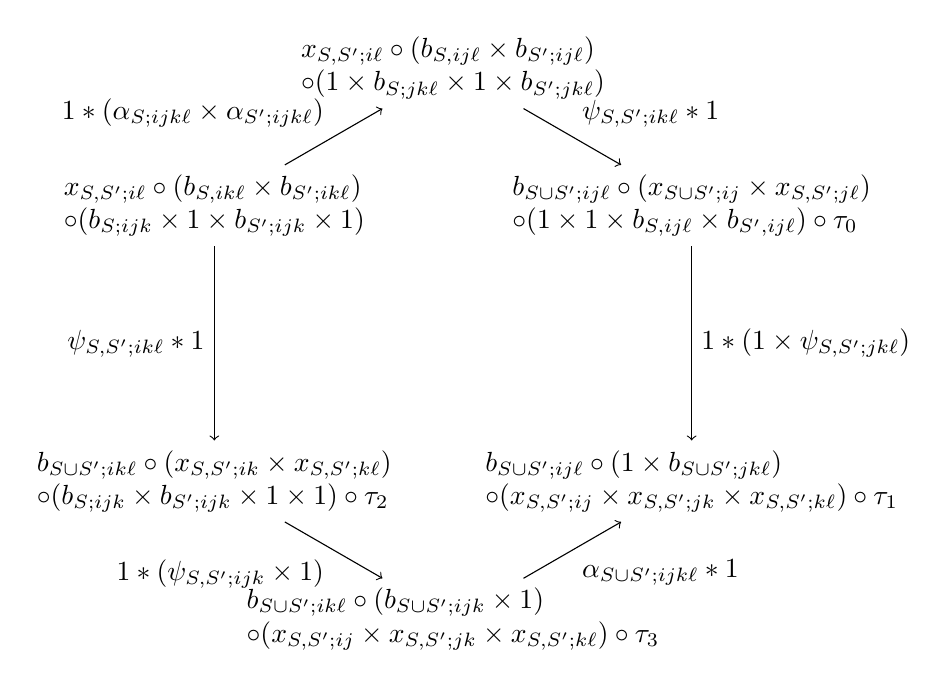
\begin{tikzpicture}[align=left]
	%		\node (A) at (126:2cm) {A};
	%		\node (B) at (54:2cm) {B};
	%		\node (C) at (342:2cm) {C}; % -18 degrees
	%		\node (D) at (270:2cm) {D};
	%		\node (E) at (198:2cm) {E};		
			\node  (A) at (150:3.5cm) {$x_{S, S'; i\ell} \circ (b_{S, ik\ell} \times b_{S'; ik\ell})$ \\ $\circ (b_{S; ijk} \times 1 \times b_{S'; ijk} \times 1)$};
			\node (B) at (90:3.5cm) {$x_{S, S'; i\ell} \circ (b_{S, ij\ell} \times b_{S'; ij\ell})$\\ $ \circ (1 \times b_{S; jk\ell} \times 1 \times b_{S'; jk\ell})$};
			\node (C) at (30:3.5cm) {$b_{S\cup S'; ij\ell} \circ (x_{S\cup S'; ij} \times x_{S, S'; j\ell}) $\\ $ \circ (1 \times 1 \times b_{S, ij\ell} \times b_{S', ij\ell} ) \circ \tau_0$}; 
			\node (D) at (330:3.5cm) {$b_{S\cup S'; ij\ell} \circ (1 \times b_{S \cup S'; jk\ell}) $\\ $ \circ (x_{S, S'; ij} \times x_{S, S'; jk} \times x_{S, S'; k\ell}) \circ \tau_1$};
			\node (E) at (270:3.5cm) {$b_{S \cup S'; ik\ell} \circ (b_{S \cup S';ijk} \times 1) $\\$ \circ (x_{S, S'; ij} \times x_{S, S'; jk} \times x_{S, S'; k\ell}) \circ \tau_3$};
			\node (F) at (210:3.5cm) {$b_{S \cup S'; ik\ell} \circ (x_{S, S'; ik} \times x_{S, S'; k \ell}) $\\$ \circ (b_{S;ijk} \times b_{S';ijk} \times 1 \times 1) \circ \tau_2$};
			\draw [->] (A) to node [above left] {$1*(\alpha_{S; ijk\ell} \times \alpha_{S'; ijk\ell})$} (B);
			\draw [->] (B) to node [above right] {$\psi_{S, S'; ik\ell}*1$} (C);
			\draw [->] (C) to node [right] {$1 * (1 \times \psi_{S,S'; jk\ell})$} (D);
			\draw [->] (A) to node [left] {$\psi_{S, S'; ik\ell}*1$} (F);
			\draw [->] (F) to node [below left] {$1 * (\psi_{S,S'; ijk} \times 1)$} (E);
			\draw [->] (E) to node [below right] {$\alpha_{S \cup S';ijk\ell} * 1$} (D);
		\end{tikzpicture}
	\end{center}
	\label{fig:EqnSSijkObject}
\end{figure}
where each $\tau_i$ represents an appropriate permutation of the factors. In other words, $(x_{S,S';-}, \psi_{S, S'; -})$ forms a structure analogous to a functor of bicategories. 
	\item  For every triple of disjoint subsets $S, S', S''$ and every 2-simplex $ijk$, the  `hexagon' equation in Figure \ref{fig:EqnSSSijObject} holds.
	\begin{figure}[ht]
		\caption{Equation for condition (TCO5) on the data of an object of $\TCfin(A,n)$.}
	\begin{center}
		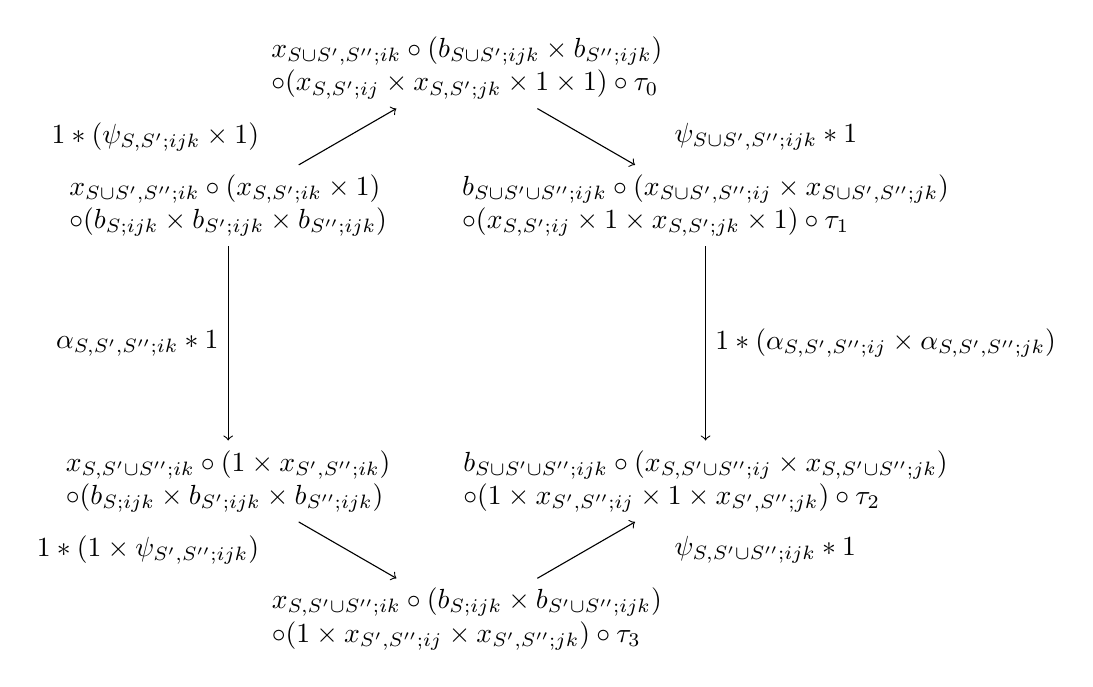
\begin{tikzpicture}[align=left]
	%		\node (A) at (126:2cm) {A};
	%		\node (B) at (54:2cm) {B};
	%		\node (C) at (342:2cm) {C}; % -18 degrees
	%		\node (D) at (270:2cm) {D};
	%		\node (E) at (198:2cm) {E};		
			\node (A) at (150:3.5cm) {$x_{S \cup S', S'';ik} \circ (x_{S, S'; ik} \times 1) $\\$\circ (b_{S;ijk} \times b_{S';ijk} \times b_{S'';ijk})$};
			\node (B) at (90:3.5cm) {$x_{S \cup S', S'';ik} \circ (b_{S\cup S'; ijk} \times b_{S''; ijk}) $\\$ \circ (x_{S, S'; ij} \times x_{S, S'; jk} \times 1 \times 1) \circ \tau_0$};
			\node (C) at (30:3.5cm) {$b_{S \cup S' \cup S''; ijk} \circ (x_{S \cup S', S''; ij} \times x_{S \cup S', S''; jk}) $\\$ \circ (x_{S, S'; ij} \times 1 \times x_{S, S'; jk} \times 1 ) \circ \tau_1$}; 
			\node (D) at (330:3.5cm) {$b_{S \cup S' \cup S''; ijk} \circ (x_{S , S' \cup S''; ij} \times x_{S,  S'\cup S''; jk}) $\\$ \circ ( 1 \times x_{S', S''; ij} \times 1 \times x_{S', S''; jk}) \circ \tau_2$};
			\node (E) at (270:3.5cm) {$x_{S, S' \cup S'';ik} \circ (b_{S;ijk} \times b_{S' \cup S''; ijk}) $\\$ \circ (1 \times x_{S', S'';ij} \times x_{S', S''; jk})  \circ \tau_3$};
			\node (F) at (210:3.5cm) {$x_{S, S' \cup S'';ik} \circ (1 \times x_{S', S''; ik} ) $\\$ \circ (b_{S;ijk} \times b_{S';ijk} \times b_{S'';ijk})$};
			\draw [->] (A) to node [left=1cm] {$1* (\psi_{S, S';ijk}\times 1)$} (B);
			\draw [->] (B) to node [right=1cm] {$\psi_{S\cup S', S''; ijk} * 1$} (C);
			\draw [->] (C) to node [right] {$1 * (\alpha_{S,S',S''; ij} \times \alpha_{S, S', S''; jk})$} (D);
			\draw [->] (A) to node [left] {$\alpha_{S, S', S'';ik}*1$} (F);
			\draw [->] (F) to node [ left=1cm] {$1 * (1 \times \psi_{S', S''; ijk})$} (E);
			\draw [->] (E) to node [right=1cm] {$\psi_{S, S' \cup S''; ijk}*1$} (D);
		\end{tikzpicture}
	\end{center}
		\label{fig:EqnSSSijObject}
	\end{figure}
	where $\tau_i$ is an appropriate permutation of the factors. 
	\item  For every quadruple of disjoint subsets $S, S', S'', S'''$, $\alpha_{-; i}$ and $\alpha_{-; ij}$ satisfy the evident pentagon equations. When $S' = \emptyset$ then $\alpha_{S, S', S''; i}$ and $\alpha_{S, S', S''; ij}$ satisfy the evident triangle identity. 
\end{list}

Let $X$ and $Y$ be two objects in $\TCfin(A,n)$. A 1-morphism from $X$ to $Y$ may only exist if each of the tensor categories agree identically $X_{S;i} = Y_{S;i}$ for each subset $S \subseteq A$ and vertex $i$ of $[n]$. In this case the 1-morphisms from $X$ to $Y$ consist of collections of data as in Table \ref{Table:1MorOfTC}.
\begin{table}[h]
	\caption{Data of a 1-morphism of $\TCfin(A,n)$.}
	\begin{tabular}{c |cccc}
	 subsets \textbackslash\ faces & vertex $i$ & edge $ij$ & 2-simplex $ijk$ & 3-simplex $ijk\ell$  \\
	\hline
	$S$ 				& n/a & $F_{S; ij}$ & $\xi_{S; ijk}$  &  (TC1M2) \\
	$S, S'$ 			& n/a & $\varphi_{S, S';ij}$ &  (TC1M3) & \\
	$S, S', S''$ 		& n/a  & (TC1M4) & & \\
	\end{tabular}
	
	\vspace{0.5cm}
	
	\begin{tabular}{l p{11cm}}
		datum & description of datum \\ \hline
		$F_{S;ij}$ & An $X_{S;i}$-$X_{S;j}$-bimodule functor from $X_{S;ij}$ to $Y_{S;ij}$. \\
		$\xi_{S;ijk}$ & A natural isomorphism of $X_{S;j}$-balanced $X_{S;i}$-$X_{S;k}$-bimodule functors from $b^Y_{S;ijk} \circ (F_{S;ij} \times F_{S; jk})$ to $F_{S;ik} \circ b^X_{S;ijk}$. \\
		$\varphi_{S,S'; ij}$ & A natural isomorphism of bilinear bimodule functors from $y_{S,S'; ij} \circ (F_{S; ij} \times F_{S';ij})$ to $F_{S \cup S'; ij} \circ x_{S, S'; ij}$. 
	\end{tabular}
	\label{Table:1MorOfTC}
\end{table}
This data is required to satisfy the following axioms:
\begin{list}{(TC1M\arabic{itemcounter})}{\usecounter{itemcounter}}
	\item If $S = \emptyset$, the $F_S;ij$ and $\xi_{S;ijk}$ are identities. If either $S$ or $S'$ is equal to $\emptyset$, then $\varphi_{S,S';ij}$ is the canonical map.
	\item For every subset $S$ and every 3-simplex $ijk\ell$ the hexagon equation in Figure \ref{fig:EqnSijklMorphism} holds.
	\begin{figure}[ht]
		\caption{Equation for condition (TC1M2) on the data of a 1-morphism of $\TCfin(A,n)$.}
		\begin{center}
			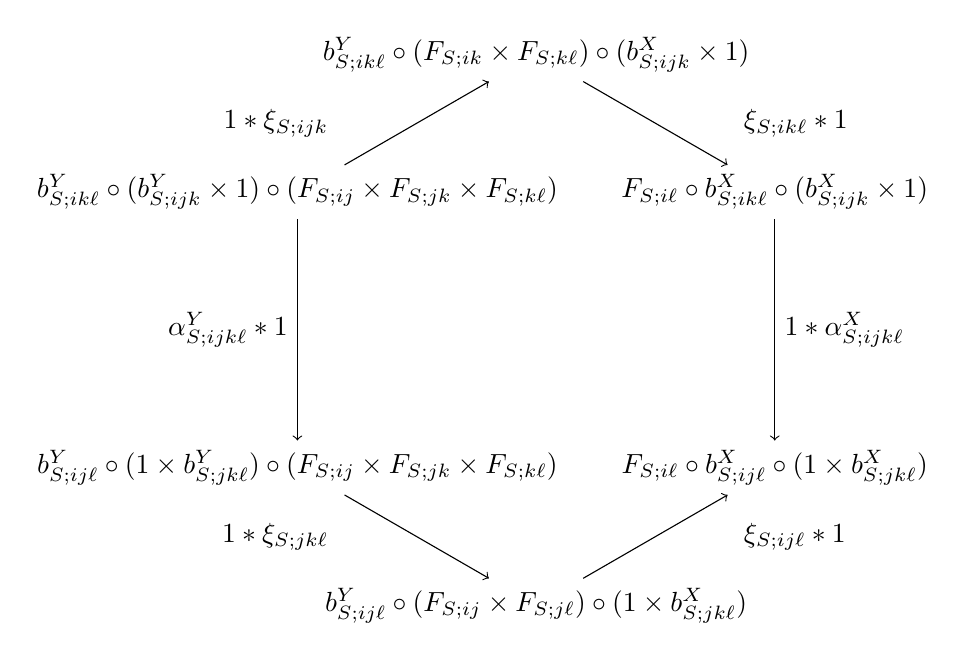
\begin{tikzpicture}[align=left]	
				\node (A) at (150:3.5cm) {$b^Y_{S;ik\ell} \circ (b^Y_{S;ijk} \times 1) \circ (F_{S;ij} \times F_{S;jk} \times F_{S;k\ell})$};
				\node (B) at (90:3.5cm) {$b^Y_{S;ik\ell} \circ (F_{S;ik} \times F_{S;k\ell}) \circ (b^X_{S;ijk} \times 1) $};
				\node (C) at (30:3.5cm) {$F_{S;i\ell} \circ b^X_{S;ik\ell} \circ (b^X_{S;ijk} \times 1)$}; 
				\node (D) at (330:3.5cm) {$F_{S;i\ell} \circ b^X_{S;ij\ell} \circ (1 \times b^X_{S;jk\ell})$};
				\node (E) at (270:3.5cm) {$b^Y_{S;ij\ell} \circ (F_{S;ij} \times F_{S;j\ell}) \circ (1 \times b^X_{S;jk\ell}) $};
				\node (F) at (210:3.5cm) {$b^Y_{S;ij\ell} \circ (1 \times b^Y_{S;jk\ell})  \circ (F_{S;ij} \times F_{S;jk} \times F_{S;k\ell})$};
				\draw [->] (A) to node [left=1cm] {$1*\xi_{S;ijk}$} (B);
				\draw [->] (B) to node [right=1cm] {$\xi_{S; ik\ell} * 1$} (C);
				\draw [->] (C) to node [right] {$1*\alpha^X_{S;ijk\ell}$} (D);
				\draw [->] (A) to node [left] {$\alpha^Y_{S;ijk\ell} * 1$} (F);
				\draw [->] (F) to node [ left=1cm] {$1*\xi_{S;jk\ell}$} (E);
				\draw [->] (E) to node [right=1cm] {$\xi_{S; ij\ell}*1$} (D);
			\end{tikzpicture}
		\end{center}
		\label{fig:EqnSijklMorphism}
	\end{figure}
	\item For every pair of disjoint subsets $S, S'$ and every 2-simplex $ijk$ the hexagon equation in Figure \ref{fig:EqnSSijkMorphism} holds, where $\tau$ permutes the middle factors. 
	\begin{figure}[ht]
		\caption{Equation for condition (TC1M3) on the data of a 1-morphism of $\TCfin(A,n)$.}
		\begin{center}
			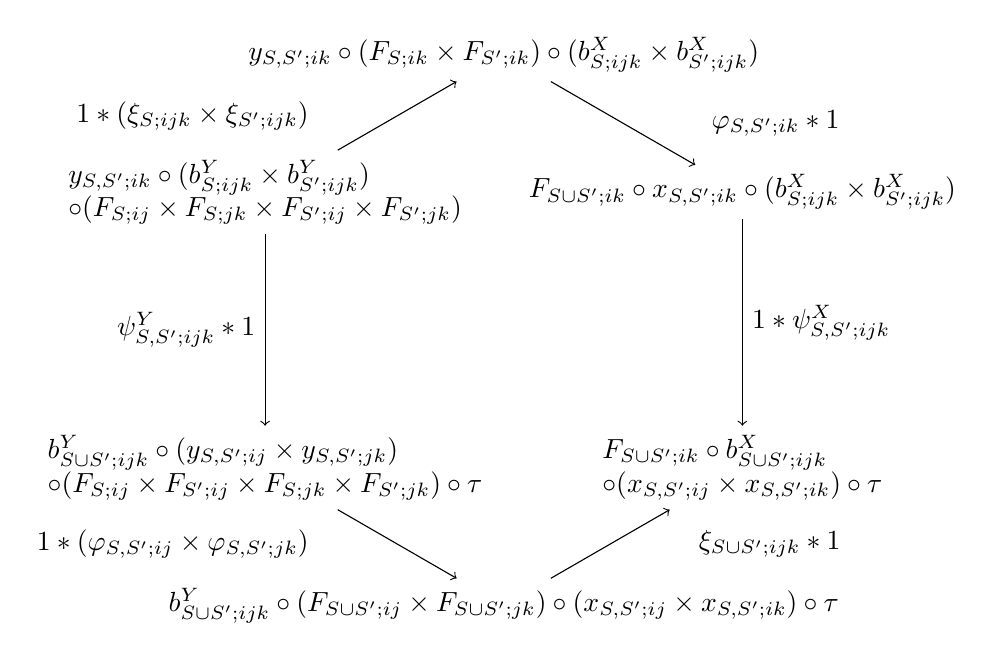
\begin{tikzpicture}[align=left]	
				\node (A) at (150:3.5cm) {$y_{S, S'; ik} \circ (b^Y_{S; ijk} \times b^Y_{S';ijk}) $\\$ \circ (F_{S; ij} \times F_{S; jk} \times F_{S'; ij} \times F_{S'; jk})$};
				\node (B) at (90:3.5cm) {$y_{S, S'; ik} \circ (F_{S; ik} \times F_{S'; ik}) \circ (b^X_{S;ijk} \times b^X_{S'; ijk}) $};
				\node (C) at (30:3.5cm) {$F_{S \cup S'; ik} \circ x_{S, S'; ik} \circ (b^X_{S;ijk} \times b^X_{S'; ijk})$}; 
				\node (D) at (330:3.5cm) {$F_{S \cup S'; ik} \circ b^X_{S \cup S'; ijk} $\\$ \circ (x_{S,S'; ij} \times x_{S,S'; ik}) \circ \tau$};
				\node (E) at (270:3.5cm) {$ b^Y_{S \cup S'; ijk} \circ (F_{S \cup S'; ij} \times F_{S \cup S'; jk}) \circ (x_{S,S'; ij} \times x_{S,S'; ik}) \circ \tau$};
				\node (F) at (210:3.5cm) {$ b^Y_{S \cup S'; ijk} \circ (y_{S,S'; ij} \times y_{S, S'; jk}) $\\$  \circ (F_{S; ij} \times F_{S'; ij} \times F_{S; jk}  \times F_{S'; jk}) \circ \tau$};
				\draw [->] (A) to node [left=1cm] {$1* (\xi_{S;ijk} \times \xi_{S';ijk})$} (B);
				\draw [->] (B) to node [right=1cm] {$\varphi_{S,S';ik}*1$} (C);
				\draw [->] (C) to node [right] {$1* \psi^X_{S, S'; ijk}$} (D);
				\draw [->] (A) to node [left] {$\psi^Y_{S, S'; ijk} * 1$} (F);
				\draw [->] (F) to node [ left=1cm] {$1* (\varphi_{S, S'; ij} \times \varphi_{S, S'; jk})$} (E);
				\draw [->] (E) to node [right=1cm] {$\xi_{S \cup S'; ijk}*1$} (D);
			\end{tikzpicture}
		\end{center}
		\label{fig:EqnSSijkMorphism}
	\end{figure} 
	\item For every triple of disjoint subsets $S, S', S''$ and every edge $ij$, the hexagon equation in Figure \ref{fig:EqnSSSijMorphism} holds.
	\begin{figure}[ht]
		\caption{Equation for condition (TC1M4) on the data of a 1-morphism of $\TCfin(A,n)$.}
		\begin{center}
			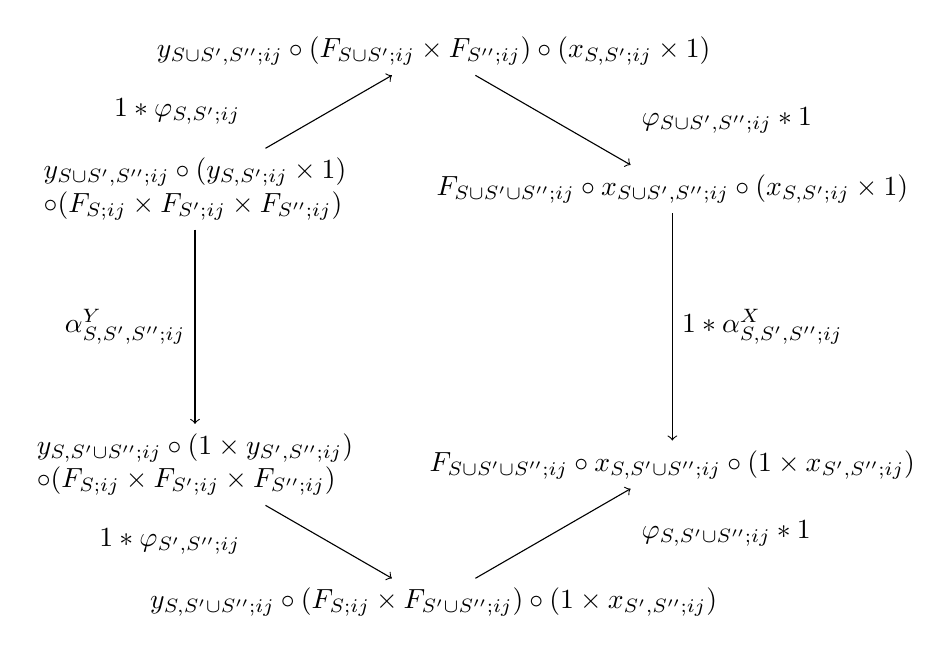
\begin{tikzpicture}[align=left]	
				\node (A) at (150:3.5cm) {$y_{S \cup S', S''; ij} \circ (y_{S, S'; ij} \times 1) $\\$ \circ (F_{S; ij} \times F_{S'; ij} \times F_{S''; ij})$};
				\node (B) at (90:3.5cm) {$y_{S \cup S', S''; ij} \circ (F_{S \cup S'; ij} \times F_{S'';ij}) \circ (x_{S,S';ij} \times 1) $};
				\node (C) at (30:3.5cm) {$F_{S \cup S' \cup S''; ij} \circ x_{S \cup S', S''; ij} \circ (x_{S,S';ij} \times 1)$}; 
				\node (D) at (330:3.5cm) {$F_{S \cup S' \cup S''; ij} \circ x_{S, S'\cup S''; ij} \circ (1 \times x_{S',S'';ij})$};
				\node (E) at (270:3.5cm) {$y_{S,  S'\cup S''; ij} \circ (F_{S;ij} \times F_{S' \cup S''; ij}) \circ (1 \times x_{S', S'';ij}) $};
				\node (F) at (210:3.5cm) {$y_{S,  S'\cup S''; ij} \circ (1 \times y_{S', S''; ij}) $\\$ \circ (F_{S; ij} \times F_{S'; ij} \times F_{S''; ij})$};
				\draw [->] (A) to node [left=1cm] {$1*\varphi_{S,S';ij}$} (B);
				\draw [->] (B) to node [right=1cm] {$\varphi_{S\cup S', S''; ij}*1$} (C);
				\draw [->] (C) to node [right] {$1 * \alpha^X_{S,S', S''; ij}$} (D);
				\draw [->] (A) to node [left] {$\alpha^Y_{S, S', S'';ij}$} (F);
				\draw [->] (F) to node [ left=1cm] {$1 * \varphi_{S', S''; ij}$} (E);
				\draw [->] (E) to node [right=1cm] {$\varphi_{S, S' \cup S''; ij}*1$} (D);
			\end{tikzpicture}
		\end{center}
		\label{fig:EqnSSSijMorphism}
	\end{figure}
\end{list}
A 2-morphism between 1-morphisms $F$ and $G$ from $X$ to $Y$ consists of a collection of $\{ \theta_{S;ij} \}$ consisting of $X_{S;i}$-$X_{S;j}$-bimodule natural transformations from $F_{S;ij}$ to $G_{S;ij}$ for each subset $S \subseteq A$ and 2-simplex $ij$ in $[n]$. For completeness we record this in Table \ref{Table:2MorOfTC}.
\begin{table}[h]
	\caption{Data of a 2-morphism of $\TCfin(A,n)$.}
	\begin{tabular}{c |ccc}
	 subsets \textbackslash\ faces & vertex $i$ & edge $ij$ & 2-simplex $ijk$   \\
	\hline
	$S$ 				& n/a & $\theta_{S; ij}$ &     (TC2M1) \\
	$S, S'$ 			& n/a &  (TC2M2)  &    \\
	\end{tabular}
%	
%	\vspace{0.5cm}
%	
%	\begin{tabular}{l p{11cm}}
%		datum & description of datum \\ \hline
%		$\theta_{S;ij}$ & An $X_{S;i}$-$X_{S;j}$-bimodule natural transformation from $X_{S;ij}$ to $Y_{S;ij}$. 
%	\end{tabular}
	\label{Table:2MorOfTC}
\end{table}
These are required to satisfy that $\theta_{\emptyset;ij}$ is the identity and the following pair of equations hold:
\begin{list}{(TC2M\arabic{itemcounter})}{\usecounter{itemcounter}}
	\item For each 2-simplex $ijk$, we have
	\begin{equation*}
		(\theta_{S; ik} * 1) \circ \xi^F_{S; ijk} = xi^G_{S;ijk} \circ (1 * (\theta_{S; ij} \times \theta_{S; jk})).
	\end{equation*}
	\item For each pair of disjoint subsets $S, S'$ we have
	\begin{equation*}
		(\theta_{S \cup S'; ij} * 1) \circ \varphi^F_{S, S'; ij} = \varphi^G_{S,S';ij} \circ (1*(\theta_{S;ij} \times \theta_{S';ij})).
	\end{equation*}
\end{list}
With these as objects, 1-morphisms, and 2-morphisms, the obvious composition makes $\TCfin(A,n)$ into a strict $2$-category. It is manifestly functorial in $A$ and $[n]$ and thus gives a (strict) functor 
\begin{equation*}
	\TCfin: \Gamma^\textrm{op} \times \Delta^\textrm{op} \to \Cat_2.
\end{equation*}
into the 1-category of strict 2-categories. Composing with the coherent nerve for strict 2-categories gives us a $\Gamma$-3-fold simplicial space, which we also denote $\TCfin$. There are two other variations on $\TCfin$ which will be of key importance. 
\begin{itemize}
	\item $\TCrig$ in which only rigid finite tensor categories appear. 
	\item $\TCsep$ in which only separable rigid finite tensor categories and separable bimodule categories appear. 
\end{itemize}



\begin{theorem}
	 $\TCfin$, $\TCrig$, and $\TCsep$ are symmetric monoidal 3-fold Segal categories.  
\end{theorem}

\CSP{This maybe needs a little more explanation...}
\begin{proof}
	Beginning with $\TCfin$,
	by Lemma \ref{lma:2catnervereflectsequiv} it is enough to show that the functor to strict 2-categories satisfies the appropriate Segal conditions, i.e. that the following Segal maps are weak equivalences of strict 2-categories:
	\begin{align*}
		\TCfin(A, m + n) & \to \TCfin(A, m) \times_{\TCfin(A, 0)} \TCfin(A, n), \\
		\TCfin(A, n) & \to \TCfin(1, n)^{\times |A|}. 
	\end{align*}
However $\TCfin$ is constructed in such a way that these Segal maps are manifestly weak equivalences. In each case the difference between the left-hand-side and the right-hand-side consists of choices of representatives of a Deligne tensor product (and maps representing the tensor product). The category of such choices is contractible (by the universal property of the Deligne tensor product) hence these Segal maps are equivalences. This argument applies equally to $\TCrig$ and $\TCsep$ as both rigidity and separability of tensor categories are preserved under the Deligne tensor product, and separability of bimodule categories is preserved  under both the Deligne tensor product and composition of bimodule categories (cf. Corollary \ref{cor:RigidityViaFunctors}, Remark \ref{rmk:rigidpreservedbytensor}, and Theorem \ref{thm:compositeOfSep}).  
\end{proof}



\CSPcomm{
\begin{itemize}
	\item . [Simpson, Lm 14.6.3, Thm 21.2.1] shows that the homotopy category of a Segal category is invariant under weak equivalence (of Segal categories in the projective (when it exists) or Reedy or injective structures).
	\item if $A$ is a sufficiently nice model category the there are a maps from $Seg_A^{proj}$ to $Seg_A^{inj}$ and then  from $Seg_A^{inj}$ to $CSS(A)$, by Lurie. (building on work of Bergner). 
	\item Wish List: A theorem that says that the various 2-categories we can extract from a symmetric monoidal $(\infty, 3)$-category are model invariant, i.e. don't change under the completion process. This would help justify the calculations we do in the sequel. 
\end{itemize}


}


%% The Bibliography
\bibliographystyle{alpha}
\bibliography{bibliography/bibliography}

\section{Dustbin}

We begin with a brief discussion of our conventions regarding duality.

%\CD{The organization of this section might well change as we decide what exactly we should include.}

%\CDcomm{Our goal is to define $\TC(3)$, ie [...].  We are not trying to include a huge discussion of all the different variations $\TC(i)$, which can occur in DTCII.}


\section{Conventions for Duality}
In this paper we ultimately consider a certain 3-category in which several different kinds of duality appear simultaneously. These dualities arise from differing mathematical points of view and so we have been tasked with finding a sensible and consistent notation in which to speak about these various forms of duality. This is no easy task as the literature has well established conventions which are at times contradictory.  The purpose of this section is to explain a compromise and clarify the conventions we will use.

There are two conventions which we perceive as fundamental: those for adjoint functors and those for rigid monoidal categories. 
\begin{definition} [Convention A]
	A functor $G: \cA \to \cB$ {\em admits a left adjoint} if there exists a functor $F: \cB \to \cA$ and natural transformations, the {\em unit} $\eta: id_{\cB} \to G \circ F$ and the {\em counit} $\varepsilon: F \circ G \to id_{\cA}$, satisfying the following pair of `zig-zag' equations:
	\begin{align*}
		(id_{G} \circledcirc \varepsilon  ) \circ (  \eta \circledcirc id_{G}) &= id_{G} \\
		(\varepsilon \circledcirc id_{F}) \circ (id_{F} \circledcirc \eta) &= id_{F}.
	\end{align*}
Here $\circledcirc$ denotes the horizontal composite of natural transformations.
We say $F$ is the {\em left adjoint} of $G$ and $G$ is the {\em right adjoint} of $F$. 
\end{definition}
With this standard convention we have a canonical natural isomorphisms $\Hom_\cA(F(x), y) \cong \Hom_\cB(x, G(y))$. 
\begin{definition} [Convention B] \label{def:rigid}
	A monoidal category $(\cC, \otimes, 1)$ is {\em rigid} if for each object $x \in \cC$, there exists an object $x^*$ and morphisms, the {\em coevaluation} $\eta: 1 \to x \otimes x^*$ and the {\em evaluation} $\varepsilon: x^* \otimes x \to 1$, satisfying the following pair of `zig-zag' equations:
	\begin{align*}
		(id_{x} \otimes \varepsilon  ) \circ (  \eta \otimes id_{x}) &= id_{x} \\
		(\varepsilon \otimes id_{x^*}) \circ (id_{x^*} \otimes \eta) &= id_{x^*}.
	\end{align*}
\end{definition}
A convenient mnemonic for this notation is to think of the $*$ as eating things. Consider the following example:
\begin{example}
	For any category $\cA$, the functor category $\Fun(\cA, \cA)$ is a monoidal category with tensor product given by composition of functors $\circ$. 
\end{example}

We impose one further convention (Convention (C)), which is that Convention (A) and Convention (B) should hold simultaneously in the above example. This forces us to consider the object $x^*$ as the {\em left adjoint} (or {\em left dual}) of $x$, despite the fact that the ``$*$'' occurs on the right of the symbol ``$x$''. 

\NScomm{[Note that there is another option.  In order to interpret $x^*$ as an adjoint, we need to interpret $x$ as a morphism and $\otimes$ as composition.  As always there are competing conventions about whether $f \otimes g$ means $f(g(-))$ or $g(f(-))$.  We were implicitly using the former convention.  If you use the latter then Conventions (A) and (B) hold, and then $x^*$ is a right dual as in EGNO and ENO.  We plan to change to this latter convention in the next reversion of the paper.]}

This has the following natural consequences:
\begin{itemize}
	\item The left dual acts on the left of the object $x$ to produce a map to the unit. 
	\item These notions extend to duals for the 2-category $Alg$ of algebras, bimodules, and bimodule maps: An $A$-$B$-bimodule $M$ with a left adjoint (or left dual) ${}_BM^L_A$ has evaluation and coevaluation maps:
	\begin{equation*}
		ev: {}_BM^L \otimes_A M_{B} \to {}_B B_B, \quad \quad coev: {}_AA_A \to {}_A M \otimes_B M^L_A.
	\end{equation*}
	\item Thus an $A$-$B$-bimodule should be considered a morphism from $B$ to $A$, for then there is a functor $Alg \to \Cat$ sending an algebra $A$ to its category $\Mod{A}{}$ of left modules, which sends left duals to left adjoint functors, and similarly for right duals. 
	\item Moreover way we typically write composition of bimodules then agrees with the way we write composition of their corresponding functors. 
\end{itemize}

If one insists on the opposite convention, calling $x^*$ the right dual of $x$, then one must also deny Convention (C) and these consequences. We end with a final well-known observation. 


\begin{remark}
	For a fixed object $x$ which admits a left dual, there is a category whose objects $(x^*, \eta, \varepsilon)$ consist of those left duals, with choices of unit and counit maps. This category is easily shown to be {\em contractible} (equivalent to the terminal category). Hence the choice of a left dual is unique up to unique isomorphism. In particular there are canonical isomorphism ${}^*(x^*) \cong ({}^*x)^* \cong x$. 
The same observation applies to adjoint functors, and duals of bimodules.  
\end{remark}

\section{Exact module categories and adjoints of module functors}
We will now specialize to the theory of finite rigid tensor categories.  The goal of this section is to summarize Etingof and Ostrik's theory of exact module categories \cite{MR2119143}.

\begin{definition}
	Let $\cC$ be a finite rigid tensor category. A (left) $\cC$-module category $\cM$ will be called {\em exact} if for any object $M \in \cM$ and  projective object $P \in \cC$, the object $P \otimes M$ is projective in $\cM$. 
\end{definition}

\begin{example}
	If $\cC$ is semisimple (e.g. $\cC = \Vect$), then $\cM$ is an exact module category if and only if it is also semisimple.
\end{example}

\begin{example}[{\cite[Example 2.6.5]{EGNO}}]
	The finite rigid tensor category $\cC$ is exact considered as a $\cC$-, $\cC^{mp}$-, or $\cC \otimes \cC^{mp}$-module category. 
\end{example}

The following omnibus theorem summarizes the key properties of exact module categories: 
\begin{theorem}[ \cite{EGNO}] \label{Thm:ExactModCatOmnibus}
	Let $\cC$ be a finite rigid tensor category, and let $\cM$, $\cM'$, $\cM''$ be exact $\cC$-module categories, and $\cN$ an arbitrary $\cC$-module category. Then,
	\begin{enumerate}
		\item $\cM$ has enough projectives \cite[Lemma 2.7.1]{EGNO}
		\item Every projective object in $\cM$  is injective, and vice versa. \cite[Cor 2.7.4]{EGNO}
		\item $\Fun_{\cC}(\cM, \cM')$ is finite \cite[Prop 2.13.5]{EGNO}; In particular $\cM \simeq \Fun_{\cC}(\cC, \cM)$ is finite.
		\item Composition $\Fun_{\cC}(\cM, \cM') \times \Fun_{\cC}(\cM', \cM'') \to \Fun_{\cC}(\cM, \cM'')$ is exact in each variable. \cite[Lemma 2.13.2]{EGNO}		
		\item Every additive (not a priori right exact) module functor $F:\cM \to \cN$ is exact \cite[Prop 2.7.8]{EGNO}. Hence every functor $F \in \Fun_{\cC}(\cM, \cM')$ is exact, and has exact left and right adjoints. Moreover, it follows that   $\Fun_{\cC}(\cM,\cM)$ is again a finite rigid tensor category. 
	\end{enumerate}
\end{theorem}

The following result is well-known, but no proof has appeared in the literature.

\begin{lemma}
	Let $\cC$ be a rigid tensor category. Then every lax (respectively oplax) $\cC$-module functor is strong.  
\end{lemma}

\begin{proof}
We do the oplax case, the lax case is similar.  Suppose that $f_{c,m}:  c \otimes \cF(m) \rightarrow \cF(c \otimes m)$ is a binatural transformation making $\cF$ into an oplax module functor.  The inverse to this natural transformation is given explicitly by the mate of $f_{c^*,m}$ 
$$\cF(c \otimes m) \rightarrow c \otimes c^* \otimes \cF(c \otimes m) \rightarrow c \otimes \cF(c^* \otimes c \otimes m) \rightarrow c \otimes \cF(m)$$
where the first map is given by the coevaluation, the second map is $f_{c^*,m}$, and the third map is evaluation.

\NScomm{[Insert diagram here]}

We need to check that this map is inverse to $f_{c^*,m}$.  This is a straightforward calculation, first use the associativity condition for module functors, and second use naturality to pull an evaluation through the natural transformation.  The following diagram illustrates this calculation.

\NScomm{[Insert diagram here]}
\end{proof}


\begin{lemma} \label{module-adjoint}
Let $\cC$ and $\cD$ be rigid tensor categories. Let  $\cM$ and  $\cN$  be  $\cC$-$\cD$-bimodule categories and let $\cF: \cM \to \cN$ be a $\cC$-$\cD$-bimodule functor.  If the underlying functor of $\cF$ has a right (respectively left) adjoint as a functor, then $\cF$ has a right (resp. left) adjoint $\cC$-$\cD$-bimodule functor. 
\end{lemma}
\begin{proof}
Suppose that $\cG$ is the right adjoint to the underlying functor of $\cF$, we will show that $\cG$ has a natural structure of a $\cC\boxtimes \cD^{mp}$-module functor.  The result for left adjoints is similar.

The binatural transformation $\psi_{x,n}: x \otimes \cG(n) \rightarrow \cG(x \otimes n)$ is given by the mate
$$x \otimes \cG(n) \rightarrow \cG \cF(x \otimes \cG(n)) \rightarrow \cG(x \otimes \cF\cG(n)) \rightarrow \cG(x \otimes n)$$
where the first map is the unit of the adjunction, the second map is the binatural transformation coming from the module functor structure on $\cF$ and the third map is the counit.  (Note that this mate rotates in the opposite direction from the one in the previous lemma.)

\NScomm{[Insert diagram here]}

Applying the previous lemma, rigidity of $\cC$ and $\cD$ guarantees that this binatural transformation is an isomorphism.  The compatibility condition is an easy exercise with commuting diagrams.
\end{proof}

\begin{remark}
If $\cC$ and $\cD$ are not rigid the above argument only shows that the right adjoint to a (lax) module functor has only an oplax module functor structure, while the left adjoint of an (oplax) module functor has only a lax module functor structure.  This is a serious issue as the following example shows. 
\end{remark}

\begin{example} \label{ex:lax-module}
	Let $\cR \cong \Vect \oplus \Vect \cdot X$ be tensor category consisting of pairs of vector spaces, which we write as $V_1 + V_2 X$, with tensor product given by 
	\begin{equation*}
		(V_1 + V_2 X) \otimes (W_1 + W_2 X) = V_1 \otimes V_2  +  (V_1 \otimes W_2 \oplus V_1 \otimes W_1)X.
	\end{equation*} 
	There are natural choices of associator and unitors making this tensor category. It is a categorification of the ring $k[x]/(x^2)$. $\cR$ is a finite semisimple tensor category, but it is not rigid. There is no object $Z \in \cR$ such that $Z \otimes X$ has a non-zero map to or from the unit object of $\cR$. Hence $X$ cannot have a dual. 
	
	There is a tensor functor $F:\cR \to \Vect$ given by $(V_1 + V_2 X) \mapsto V_1$. This gives the category $\Vect$ the structure of a (left) $\cR$-module category, and moreover $F$ is naturally an $\cR$-module map. $F$ has both a left and right adjoint, which agree and are given by the functor $G: \Vect \to \cR$ sending $W \in \Vect$ to $(W + 0 X) \in \cR$. It is not possible to give $G$ the structure of an $\cR$-module functor. 
\end{example}

\section{Separable Module Categories} \label{sec-tc-separable}

In this section we introduce a new notion of separability for algebra objects, module categories, and tensor categories.  This theory is a generalization of the classical notion of a separable algebra.  The main point of this notion is to provide the right generalization of certain results to fields of characteristic $p$.  In particular, it gives the right generality for M\"uger's result on semisimplicity of the center of a semisimple category \cite[Theorem 3.16]{MR1966525} and Etingof--Nikshych--Ostrik's result on semisimplicity of categories of functors between fusion categories \cite[Theorem 2.16]{MR2183279}.  Furthermore, it also allows us to avoid an issue related to inseparable extensions pointed out by Kuperberg \cite[Question 5.1]{MR1995781}.  This section was inspired by a suggestion of Ostrik, and by the appearance of separability in the classification of $2$-dimensional local field theories \cite{schommer-pries-thesis}.

\NScomm{This section is still under construction.}

\begin{definition}
	Let $A$ be an algebra object in a finite tensor category $\cC$. The multiplication map $\mu: A \otimes A \to A$ may be viewed as a morphism of $A$-$A$-bimodule objects in $\cC$. We will say that $A$ is {\em separable} if the multiplication map splits as a map of $A$-$A$-bimodules. 
\end{definition}

\begin{remark}
	A (right exact) monad $T$ acting on a $\cC$-module category $\cM$ is an algebra object in the tensor category $\Fun_\cC(\cM, \cM)$. Thus the above definition also yields the notion of {\em separable monad}. 
\end{remark}

\begin{remark}
	When $\cC = \Vect_k$, then a separable algebra $A$ is separable in the classical sense. Over a perfect field --- such as a finite field, an algebraically closed field, or a field of characteristic zero --- this is equivalent to $A$ being a finite dimensional semisimple $k$-algebra; more generally it is a stronger condition. 
	\CSP{get references to classical notion of separability}
\end{remark}

\begin{theorem} \label{thm:SepModCats}
	Let $\cC$ be a finite semisimple tensor category (not necessarily rigid) and let $\cM$ be a finite right $\cC$-module category. Then the following are equivalent:
	\begin{enumerate}
		\item $\cM_\cC \simeq \Mod{A}{}(\cC)$, where $A$ is a separable algebra in $\cC$;
		\item $\cM_\cC \simeq \Mod{A}{}(\cC)$, where $A$ is an algebra in $\cC$ which is projective as an $A$-$A$-bimodule;
		\item The identity functor is a projective object of $\Fun_\cC(\cM, \cM)$;
		\item $\Fun_\cC(\cM, \cM)$ is a semisimple category. 
	\end{enumerate}
	Moreover if any of these conditions is satisfied, then $\cM$ is semisimple, hence exact as a $\cC$-module category. The analogous results hold for left $\cC$-module categories as well. 
\end{theorem}


\begin{proof}
	The last sentence is clear since we may switch left/right actions by taking the monoidally-opposite category.
	The proof of Lemma \ref{Lma:FunctorsAsATensorPdt} shows that $\Fun_\cC(\cM, \cM) \simeq \Mod{A}{A}(\cC)$, thus we have clear implications (4) $\Rightarrow$ (3) $\Leftrightarrow$ (2) $\Rightarrow$ (1). We will show that (1) $\Rightarrow$ (4), that is if $A$ is separable, then $\Mod{A}{A}(\cC)$ is a semisimple category. 
	
	To see this, recall the following general fact: if $F: \cA \leftrightarrows \cB: G$ is an adjunction between abelian categories and the right adjoint $G$ is also right exact, then $F$ sends projective objects to projective objects. This is clear as
	\begin{equation*}
		\Hom(F(P), -) \cong \Hom(P, U(-))
	\end{equation*}
	is a right-exact functor. In particular this applies to the free-forget adjunction between $A$-$A$-bimodules and objects of $\cC$. As every object of $\cC$ is projective (since it is semisimple) we have that every free $A$-$A$-bimodule is also projective in $\Mod{A}{A}(\cC)$. 
	
Let $s: {}_AA_A \to {}_AA \otimes A_A$ be a bimodule splitting of the multiplication map. For every $A$-$A$-bimodule $X$ we have an induced $A$-$A$-bimodule map
\begin{equation*}
	X \cong A \otimes_A X \otimes_A A 
	\xra{s \otimes_A 1 \otimes_A s} (A \otimes A) \otimes_A X \otimes_A (A \otimes A) \cong A \otimes X \otimes A,
\end{equation*}  	
which splits the canonical action map. Thus $X$ is a direct summand of the free bimodule $A \otimes X \otimes A$. As this latter is projective, $X$ is projective. Thus $\Mod{A}{A}(\cC)$ is semisimple, and (1) $\Rightarrow$ (4). 
	
Similarly if $Y \in \cM \simeq \Mod{A}{}(\cC)$ is a left $A$-module, then $s \otimes_A 1: Y \cong A \otimes_A Y \to (A \otimes A) \otimes_A Y \cong A \otimes Y$ realizes $Y$ as a direct summand of a free $A$-module. Again since $\cC$ is semisimple, free $A$-modules are necessarily projective. Thus $Y$ is projective. Hence $\cM$ itself is semisimple.  	
\end{proof}

\begin{definition}
	If any of the equivalent conditions of Theorem \ref{thm:SepModCats} are satisfied, then we will say that $\cM$ is a {\em separable} module category. If $\cM$ is a $\cC$-$\cD$-bimodule category then we will say $\cM$ is separable if it is separable over both $\cC$ and $\cD$ separately. 
\end{definition}

\begin{theorem} \label{thm:compositeOfSep}
	If ${}_\cB\cM_\cC$ and ${}_\cC\cN_\cD$ are separable bimodule categories over semisimple tensor categories, then $\cM \boxtimes_{\cC} \cN$ is a separable $\cB$-$\cD$-bimodule category.
\end{theorem}

\begin{proof}
	As separability is a condition on each module structure separately, is is enough to check that $\cM \boxtimes_{\cC} \cN$ is a separable as a $\cB$-module category. Our assumptions give the following identifications:
\begin{itemize}
	\item $\cM \simeq \Mod{}{A}(\cB)$ as left $\cB$-module categories for a separable algebra $A$ in $\cB$;
	\item $\cM \simeq \Mod{B}{}(\cC)$ as right $\cC$-module categories for a separable algebra $B$ in $\cC$;
	\item $\cN \simeq \Mod{}{C}(\cC)$ as left $\cC$-module categories for a separable algebra $C$ in $\cC$;
	\item $\cM \boxtimes_{\cC} \cN \simeq \Mod{B}{C}(\cC)$
\end{itemize}
Thus $\cM \boxtimes_{\cC} \cN$ is equivalent to the category of algebras for the separable monad $T = (-) \otimes C$ acting on $\cM$. Moreover $T$ is an algebra (monad) in $\Fun_{\cB}(\cM, \cM)$ (this follows as the left $\cB$-action on $\cM$ commutes up to coherent natural isomorphism with the right $\cC$-action), and this induces the structure of an algebra on the object $T(A) \in \cB$. The multiplication is given by,
\begin{equation*}
	T(A) \otimes T(A)  \simeq T( T(A) \otimes A)  \xra{T(\textrm{action})} T^2(A) \to T(A),
\end{equation*}
where the first equivalence comes from left $\cB$-linearity of $T$, the next map comes from the action map on $T(A)$ ($T(A) \in \cM \simeq \Mod{}{A}(\cB)$ has a right $A$-action), and the final map is one of the structure maps of the monad $T$. The unit of $T(A)$ is defined similarly. 

One readily verifies that the the unit map $A \to T(A)$ is an homomorphism of algebras in $\cB$. Moreover as $T$ is right exact and $\cB$-linear, we have $T(m) \cong m \otimes_A T(A)$ for all $m \in \Mod{}{A}(\cB) \simeq \cM$. Thus the category of $T$-algebras in $\Mod{}{A}(\cB)$ is nothing more then the category of right $T(A)$-modules in $\cB$.  Hence we have shown $\cM \boxtimes_{\cC} \cN \simeq \Mod{}{T(A)}(\cB)$ as left $\cB$-module categories. It remains to show that $T(A)$ is a separable algebra in $\cB$.

As both $A$ and $T$ are separable, we have splittings of the canonical multiplication maps, $s: A  \to A \otimes A$, and $\sigma:T \to T^2$. These induce a splitting of the $T(A)$-multiplication map:
\begin{equation*}
	T(A) \stackrel{\sigma}{\to} T^2(A) \xra{T(1 \otimes_A s)} T( T(A) \otimes A) \cong T(A) \otimes T(A).
\end{equation*}
Thus $T(A)$ is separable.
\end{proof}

\begin{definition}
	A tensor category is {\em separable} if it is separable as a $\cC \boxtimes \cC^\mp$-$\Vect$-bimodule category.  
\end{definition}

\begin{definition}
	Let $\cC$ be a finite tensor category. The {\em center} of $\cC$ is the linear category $\cZ(\cC) \simeq \Fun_{\cC \boxtimes \cC^\mp}(\cC, \cC)$.
\end{definition}

\begin{corollary}
	The following are equivalent for a finite tensor category $\cC$ which is $\Vect$-separable.
	\begin{enumerate}
		\item $\cC$ is separable;
		\item The center $\cZ(\cC)$ is semisimple.
	\end{enumerate} 
\end{corollary}

\CSPcomm{[Add some closure properties for separable. Example: the external Deligne tensor product of separable bimodules, the tensor product of separable tensor categories, functor categories, etc.]}



\section{Fusion categories} \label{sec-tc-fusion}.%!%remove period

\NScomm{[This section is under construction]}

\begin{definition}
A \emph{fusion category} is a tensor category $\cC$ over $k$ satisfying the following conditions:
\begin{enumerate}
\item $\cC$ is finite.
\item $\cC$ is rigid. 
\item $\cC$ is semisimple. 
\end{enumerate}
\end{definition}

Thus a fusion category has finite dimensional hom vector spaces, has finitely many isomorphism classes of simple objects, and for every object $a \in \cC$ there exists an object ${a^*} \in \cC$ that is a left dual for $a$ and also an object ${}^{*}a \in \cC$ that is a right dual for $a$.

\begin{warning}
Here for brevity we use ``fusion category" to refer to what has elsewhere gone under the name ``multi-fusion category". In particular we do not assume that the unit object is simple.  Furthermore we only assume semisimplicity, not split semisimplicity.
\end{warning}

We quickly recall several lemmas relating fusion categories to the notions in the last two sections.

\begin{lemma}
If $\cC$ is fusion, then a module category $\cM$ over $\cC$ is exact if and only if it is semisimple.
\end{lemma}

\begin{definition}
If $\cC$ is a fusion category we define its global dimension to be \NScomm{[figure out what the best definition is for the argument, and make sure that it makes sense when the unit is not simple]}
\end{definition}

\begin{proposition}
A fusion category of non-zero global dimension is separable. \CSPcomm{[add references/sketch of the proof.]}
\end{proposition}

---------

\CSPcomm{ [remove this...] 
Given a monoidal category $\cC$, there are three important notions of opposite. We can reverse the order of tensor product, reverse the order of composition, or reverse both.  We will denote these $\cC^{\op}$ (the opposite category), $\cC^{\mp}$ (the monoidally-opposite category), and $\cC^{\mop}$ (the opposite monoidally-opposite category).  (Note that in the literature $\op$ sometimes refers to what we call $\op$ and sometimes to what we call $\mp$, also in the literature $\mp$ is also denotes $rev$.)
%We will denote by $\cC^{\op}$ the monoidal category whose underlying category is opposite to the underlying  category of $\cC$, and whose monoidal structure is inherited from the monoidal structure of $\cC$; we call it the {\em opposite monoidal category}.  By contrast, we will let $\cC^{\mp}$ denote the monoidal category whose underlying category is the underlying category of $\cC$, and whose monoidal structure is defined by $[a] \otimes [b] := [b \otimes a]$, where $[a]$ refers to the object $a \in \cC$ viewed as an object of $\cC^{\mp}$; we call this the {\em monoidal opposite category}.  Finally, there is $\cC^{\mop}$, which denotes the monoidal category whose underlying  category is $\cC^{\op}$ and whose monoidal structure is inherited from the monoidal structure of $\cC^{\mp}$; we call this the {\em opposite monoidal opposite category}.


%%%%%%%%%%%
%
%  Here is where the definition of left/right duals and rigidity were initially. 
%
%%%%%%%%%%%%

%\begin{definition}
%	A monoidal category is {\em rigid} if every object admits both left and right duals (cf. Def. \ref{def:duals}).
%\end{definition}


\begin{lemma} \label{lma:RigidIsExact}
	Let $(\cC, \otimes)$ be a rigid tensor category (cf. Def. \ref{def:rigid}). Then the multilinear functor $\otimes: \cC \times \cC \to \cC$ is exact in both variables. 
\end{lemma}

\begin{proof}
	The units and counits give rise to natural isomorphisms %\NS{Currently we have both $\Hom$ and $\Hom$ in the paper.  We should pick one.}
 \begin{equation*} 
 	\Hom(x \otimes y, z) \cong \Hom( x, z \otimes y^*) \cong \Hom(y, {}^*x \otimes z).
 \end{equation*}
	Hence for all $x$ and $y$ the functors $(-)\otimes x$ and $y \otimes (-)$ admit both left and right adjoints, and are consequently exact. 
\end{proof}

\begin{corollary}
	A rigid tensor category $\cC$ is semisimple if and only if $1 \in \cC$ is a projective object. 
\end{corollary}

\begin{proof}
	If $\cC$ is semisimple if and only if every object is projective, in particular the unit object. Conversely, if $1 \in \cC$ is projective, then $\Hom(P, -) = \Hom( 1, (-) \otimes P^*)$ is an exact functor for all $P$. Hence every object is projective.  
\end{proof}

\begin{lemma}
	The assignments $x \mapsto x^*$ and $x \mapsto {}^*x$ gives rise to equivalences of rigid tensor categories $(-)^*: \cC \to \cC^{mop}$ and ${}^*(-): \cC \to \cC^{mop}$. Consequently the assignment $x \mapsto x^{**}$ gives an autoequivalence of any rigid tensor category. 
\end{lemma}

%\begin{proposition}
%If $\cC$ is a fusion category, then there exist monoidal functors $\ld{(-)} : \cC \ra \cC^{\mop}$ and $\rd{(-)} : \cC \ra \cC^{\mop}$ whose values on any object $a \in \cC$ are respectively a left dual object $\ld{(a)}$ and a right dual object $\rd{(a)}$ for $a$.
%\end{proposition} \CD{This proposition doesn't actually depend on fusion, right?  Should change the statement so that only what is needed (existence of duals) is assumed.}

\begin{proof}
Let $\otimes$ denote the tensor product on $\cC$ and $\cdot$ the tensor product on $\cC^{\mop}$, so that $x \cdot y = y \otimes x$.

First we construct the functor ${(-)^*}$.  Define ${(-)^*}$ on objects by picking for each object $a \in \cC$ a left dual object ${a^*} \in \cC$.  Also pick a unit map $\eta_a: 1 \ra a \otimes {a^*}$ and a counit map  $\varepsilon_a: {a^*} \otimes a \ra 1$  giving ${a^*}$ the structure of a left dual to $a$.  Define the functor ${(-)^*}$ on a morphism $f: a \ra b$ to be its {\em mate}: 
\begin{equation*}
	{(f)^*} := (\varepsilon_b \otimes \id_{\rd{a}}) (\id_{\rd{b}} \otimes f \otimes \id_{\rd{a}}) (\id_{\rd{b}} \otimes \eta_a).
\end{equation*}

Next we want to construct a monoidal functor structure on $(-)^*$, that is we need natural transformations $f_{a,b}: (a \otimes b)^* \rightarrow a^* \cdot b^* = b^* \otimes a^*$.  Since the left dual is unique up to unique isomorphism, it is enough to check that $b^* \otimes a^*$ is a left dual to $b \otimes a$.  Observe that the morphisms $\rd{b} \otimes \rd{a} \otimes a \otimes b \xra{\varepsilon_a} \rd{b} \otimes b \xra{\varepsilon_b} 1$ and $1 \xra{\eta_a} a \otimes \rd{a} \xra{\eta_b} a \otimes b \otimes \rd{b} \; \rd{a}$ show that $(\rd{b} \otimes \rd{a})$ is a left dual to $(a \otimes b)$.  There is therefore a uniquely determined isomorphism from $(\rd{b} \otimes \rd{a})$ to $\rd{(a \otimes b)}$.  It is straightforward to check that this satisfies the necessary hexagon relation.

The right dual functor is analogous.  Since the left and right duals are quasi-inverse to each other, they're each equivalences.
% In principle, need to check naturality and hexagon for those isos.
\end{proof}
\begin{remark}
Applying this theorem to $\cC^{\op}$ shows that the left dual and the right dual each give monoidal equivalences between $\cC^{\op}$ and $\cC^{\mp}$.  Nonetheless, these equivalences are not canonical (indeed there are two natural choices), so we will always be careful to distinguish  $\cC^{\op}$ and $\cC^{\mp}$.
\end{remark}

\begin{corollary} \label{cor:RigidityViaFunctors}
	A tensor category $(\cC, \otimes, 1)$ is rigid if and only if there exists an equivalence of tensor categories ${{}^*(-)}: \cC \to \cC^\mp$ and natural isomorphisms
	\begin{align*}
		\Hom( {}^*y, z) &\cong \Hom(1, z \otimes y) \\
		\Hom(z, y) & \cong \Hom(z \otimes {}^*y, 1).
	\end{align*}
\end{corollary}

\begin{proof}
	It is clear from the previous lemma that a rigid tensor category admits such a structure (the natural isomorphisms in question are induced by the evaluation and coevaluation). Conversely, if we are given such a structure, then applying the above natural isomorphisms in the cases $z={}^*y$ and $y$ yield evaluation and coevaluation maps demonstrating ${}^*y$ as the right dual of $y$. Left duals are obtained by the same argument applied to the inverse of the functor ${}^*(-)$.
\end{proof}

% This fact is asserted in Bruce's thesis; the functor part is mentioned in Selinger Eg 4.4.


%\begin{remark}
%The monoidal functor $\ld{(-)}: \cC \ra \cC^{\mop}$ is an equivalence of tensor categories; the inverse functor is $\rd{(-)}: \cC^{\mop} \ra \cC$.
%\end{remark}

}



\end{document}


